% kapitel3.tex
\tikzstyle{funtool}=[blue ,line  width =1pt]
\tikzstyle{ur}=[draw, text centered, color=blue, minimum height=0.01em]
\definecolor{light-gray}{gray}{0.93}
\newcommand{\fun}[3]{%
	\path [dashedline] (#1.east) -- node [above]
	{\scriptsize #2} (#3);}
\chapter{Implementierung} \label{sec:alg}
Für das in Python implementierte RAD-Sequencing-Tool, NodeRAD, wurde zur Workflowintegration das Workflow Management System Snakemake verwendet ~\cite{koester_2012_1, koester_2012_2}. Die einzelnen Analyseschritte werden dabei über Regeln abgebildet. Für jede Regel können neben dem zu verwendenden Script oder Shell-Kommando sowie den Pfadangaben für In- und Output auch zusätzliche Optionen festgelegt werden. Dazu gehören beispielsweise Angaben zu Parametern bzw. Argumenten für die verwendeten Tools, Pfadangaben für Log-Dateien oder die Anzahl der zu verwendenden Threads. \\

Als Input benötigt der Workflow eine Datei im FASTQ-Format (siehe Kap. \ref{subsec:fastq}), welche die single-end Reads der verschiedenen Individuen mit ihren IDs, der Basensequenz und Angaben zur Basenqualität enthält. Des Weiteren ist eine Tabelle im tsv-Format erforderlich, in der die Zuordnung der Probennamen zu den Individuen und ihren Barcode-Sequenzen definiert ist. Nach dem Preprocessing, der Qualitätskontrolle der Reads und dem Sequenzalignment erfolgt die RAD-Seq-Analyse durch NodeRAD. Hierbei werden die Wahrscheinlichkeiten der Allele-Fractions und der möglichen Loci bestimmt. Die Loci mit der höchsten Wahrscheinlichkeit werden schließlich mit den Sequenzen ihrer Allele in einer Datei im Variant Call Format (VCF) ausgegeben.

\section{Preprocessing} \label{sec:preproc}
\begin{figure}[h]
	\begin{center}
		\begin{tikzpicture}[scale=0.64,transform shape]
		% https://github.com/PetarV-/TikZ/tree/master/DNA
		\path \ioitem {1}{Reads\\
			\begin{tikzpicture}[scale=0.6,transform shape]
			\bond{red}{blue}{0.1}
			\bond{red}{blue}{0.25}
			\bond{red}{blue}{0.4}
			\bond{blue}{red}{1.1}
			\bond{blue}{red}{1.25}
			\bond{blue}{red}{1.4}
			\bond{red}{blue}{2.1}
			\bond{red}{blue}{2.25}
			\bond{red}{blue}{2.4}
			\bond{blue}{red}{3.1}	
			\bond{blue}{red}{3.25}
			\bond{blue}{red}{3.4}
			\bond{red}{blue}{4.1}
			\bond{red}{blue}{4.25}
			\bond{red}{blue}{4.4}
			\braid[rotate=90,style strands={1}{red, very thick},style strands={2}{blue, very thick}] (tst) at (0, 0) s_1 s_1 s_1 s_1 ;
			\end{tikzpicture}
		};
		\path (p1.south)+(-2.5,-2.0) \blockitem{2}{\hyperref[schritt1txt]{\color{green!40}..}1. Adapter trimming};\phantomsection\label{schritt1}
		\path (p2.south)+(2.5,-1.2) \blockitem{3}{\hyperref[schritt2txt]{\color{green!40}..}2.\phantomsection\label{schritt2} Quality \\control};
		\path (p3.south)+(-2.5,-1.2) \blockitem{5}{\hyperref[schritt3txt]{\color{green!40}..}3.\phantomsection\label{schritt3} Sequence alignment};
		\path (p3.east)+(+4.4, 1.801) node (ur1)[ur] {\color{black}Cutadapt};
		\path (p1.east)+(+5.0,-4.42) node (ur2)[ur] {\color{black}FastQ, MultiQC};
		\path (p2.east)+(+7.0,-3.59) node (ur3)[ur] {\color{black}Minimap2};
		
		
		% Pfeile
		\path [line] (p1.south) -- +(0.0,-0.5) -- +(-2.5,-0.5) -- node [above, midway] {} (p2);
		\path [line] (p1.south) -- +(0.0,-0.5) -- +(+2.83,-0.5) -- node [above, midway] {} (p4);
		\path [line] (p2.south) -- node [above] {} (p3) ;
		\path [line] (p3.south) -- node [above] {} (p5) ;
		
		
		\draw [funtool] (p2) -- (ur1);
		\draw [funtool] (p3) -- (ur2);
		\draw [funtool] (p5) -- (ur3);
		
		\background{p3}{p2}{p3}{p5}{Preprocessing}
		
	\end{tikzpicture}
	\caption{Prozesse des Workflows - Preprocessing \cite{tikz_schema, tikz_dna}}
	\label{fig:workflow_all}
\end{center}
\end{figure}

Im Preprocessing werden durch das Tool Cutadapt ~\cite{martin_2011} die Reads jedes Individuums anhand ihrer Barcodesequenzen identifiziert und extrahiert (Demultiplexing). Hiernach werden die Barcodesequenzen entfernt (\hyperref[step15]{Trimming\phantomsection\label{schritt1txt}}) und die Reads jedes Individuums in separaten Dateien im FASTQ Format abgelegt. \\

Im Anschluss an das Trimming erfolgt eine \hyperref[schritt2]{Qualitätskontrolle\phantomsection\label{schritt2txt}} durch das Tool FastQC  ~\cite{andrews_2012}. Dabei werden einige allgemeine Statistiken zu den Rohdaten der Reads generiert, wie beispielsweise zur Basenqualität, zum GC-Gehalt, dem Anteil an Duplikaten oder überrepräsentierten Sequenzen. Durch das Tool MultiQC ~\cite{ewels_2016} wird aus diesen Statistiken und den Log-Dateien von Cutadapt ein Report im HTML-Format mit diversen Plots zur Veranschaulichung erstellt.

\section{Edit-Distanzen} \label{sec:edit}

Für die spätere Konstruktion eines Graphen basierend auf den Edit-Distanzen zwischen den Readsequenzen wird für jedes Individuum zunächst ein \hyperref[schritt3]{Sequenzalignment\phantomsection\label{schritt3txt}} (vgl. Kap. \ref {subsec:samformat}) mit Hilfe des Tools Minimap2 ~\cite{li_2018} erstellt. Hierbei werden alle Readsquenzen paarweise mit einander verglichen. Das Ergebnis des Mappings wird anschließend durch Samtools-view ~\cite{li_2009} in das BAM-Format konvertiert und enthält neben den Angaben zur Query- und Referenzsequenz auch den CIGAR-String sowie den NM-Tag mit den Edit-Distanzen. Der CIGAR-String und der NM-Tag definieren wichtige Kanteneigenschaften des späteren Graphen. \\

\section{Konstruktion des Graphen} \label{sec:graph}

\begin{figure}[h]
	\begin{center}
		\begin{tikzpicture}[scale=0.64,transform shape]
		% https://github.com/PetarV-/TikZ/tree/master/DNA
		\path +(1.33,-6.2) \ioitem {1}{Reads\\
			\begin{tikzpicture}[scale=0.6,transform shape]
			\bond{red}{blue}{0.1}
			\bond{red}{blue}{0.25}
			\bond{red}{blue}{0.4}
			\bond{blue}{red}{1.1}
			\bond{blue}{red}{1.25}
			\bond{blue}{red}{1.4}
			\bond{red}{blue}{2.1}
			\bond{red}{blue}{2.25}
			\bond{red}{blue}{2.4}
			\bond{blue}{red}{3.1}	
			\bond{blue}{red}{3.25}
			\bond{blue}{red}{3.4}
			\bond{red}{blue}{4.1}
			\bond{red}{blue}{4.25}
			\bond{red}{blue}{4.4}
			\braid[rotate=90,style strands={1}{red, very thick},style strands={2}{blue, very thick}] (tst) at (0, 0) s_1 s_1 s_1 s_1 ;
			\end{tikzpicture}
		};
		\path (p3.south)+(-3.0,-1.2) \ioitem{5}{3. Sequence alignment};
		\path (p3.west)+(3.25,-3.8) \blockitem{4}{\hyperref[schritt4txt]{ 4}.\phantomsection\label{schritt4} Build graph};
		\path (p4.south)+(0.0,-1.5) \blockitem{6}{\hyperref[schritt5txt]{\color{green!40}..}5.\phantomsection\label{schritt5} Connected components};
		
		\path (p4.east)+(+3.5,0) node (ur2)[ur] {\color{black}graph-tool};
		\path (p6.east)+(+3.5,0) node (ur3)[ur] {\color{black}graph-tool};		
		\path (p6.south)+(0.0,-1.4) \ioitem{8}{6. Candidate \\alleles};
	
		% Pfeile		
		\path [line] (p1.south) -- node [above, midway] {} (p4);	
		\path [line] (p5.south) -- +(0.0,-1.415) -- node [above, midway] {} (p4.west);		
		\path [line] (p4.south) --node [above] {} (p6);
		\path [line] (p6.south) -- node [above, midway] {} (p8);
		
		\draw [funtool] (p4) -- (ur2);
		\draw [funtool] (p6) -- (ur3);
		
		\background{p3}{p4}{p4}{p6}{Graph \\construction}
	\end{tikzpicture}
	\caption{Prozesse des Workflows - Konstruktion des Graphen \cite{tikz_schema, tikz_dna}}
	\label{fig:workflow_all}
\end{center}
\end{figure}

NodeRAD benötigt als Input zu jedem Individuum die getrimmten single-end Reads sowie das Sequenzalignment. Zur \hyperref[schritt4]{Konstruktion des Graphen\phantomsection\label{schritt4txt}} wird die Python-Library graph-tool ~\cite{peixoto_2014} genutzt. Zunächst wird daraus für jedes Individuum ein eigener, gerichteter Graph $ G $ mit $ G = (V,E) $ erstellt. Seine Knoten, $ V $, werden durch die einzelnen Reads repräsentiert. Entsprechend ergeben sich die Knoteneigenschaften aus den Daten der Reads, diese werden den FASTQ-Dateien nach Ausführung von Cutadapt (siehe Kap. \ref{sec:preproc}) entnommen. Die Kanten, $ E $, zwischen den Knoten ergeben sich aus dem Vergleich ihrer Sequenzen im Rahmen des Sequenzalignments mittels Minimap2 (siehe Kap. \ref{sec:edit}).\\

Zusätzlich entnimmt NodeRAD der Konfigurationsdatei des Workflows einige Konstanten und Grenzwerte für die späteren Berechnungen. Zu den Konstanten gehören die Sequenzierfehlerraten für Indels, die Heterozygotiewahrscheinlichkeiten für Substitutionen, Insertionen und Deletionen sowie die Ploidie des Chromosomensatzes der untersuchten Spezies. Diese werden im Script \lstinline|noderad_main.py| im Graphen als Grapheigenschaften abgelegt. Als konfigurierbare Grenzwerte gibt es für NodeRAD einen Schwellenwert \linebreak \lstinline|edit-distance-graph| für die maximal zulässige Edit-Distanz, bei der zwei Knoten noch durch eine Kante verbunden werden sowie Schwellenwerte zum Filtern selten vorkommender Sequenzen (\lstinline|treshold-seq-noise| für \lstinline|small-clusters| und \lstinline|large-clusters|) ober- und unterhalb einer bestimmten Clustergröße (\lstinline|treshold-cluster-size|), die als Hintergrundrauschen nicht in der Berechnung Berücksichtigung finden sollen. \\

\subsection{Knoten des Graphen} \label{subsec:nodes}

Die Knoten werden aus den FASTQ-Daten der getrimmten Reads mittels SeqIO aus der Library Biopython ~\cite{cock_2009_1} ausgelesen und im Graphen mit den Knoteneigenschaften ihrer Basensequenz, einer internen ID sowie Angaben zur Basenqualität abgelegt. Die Codierung des Qualitystrings der Reads variiert je nach verwendeter Plattform. Daher wird er durch SeqIO ausgelesen und für jede Base in ein einheitliches Maß, den Phred Quality Score, decodiert ~\cite{cock_2009_2}. Für jeden Knoten werden die Vektoren mit den Phred Qualitiy Scores der Basen als Knoteneigenschaft gespeichert. \\

\subsection{Kanten des Graphen} \label{subsec:edges}
Die Kanten des Graphen definieren sich durch die mittels Minimap2 erzeugten Sequenzalignments (vgl. Kap. \ref{sec:edit}). Jedes Alignment zweier Reads entspricht im Graphen einer gerichteten Kante $e = (source,\; target)$, die den Vergleich der Query- zur Referenzsequenz repräsentiert. Sie verbindet somit zwei der zuvor aus der FASTQ-Daten erzeugten Knoten. Das Auslesen des Alignmentfiles im BAM-Format erfolgt mit Hilfe der Python-Library pysam ~\cite{pysam}. Dabei werden die Edit-Distanzen aus dem NM-Tag genutzt, um nur Kanten in den Graphen aufzunehmen, die unterhalb des durch die Konfigurationsdatei festgelegten Grenzwertes \lstinline|threshold_max_edit_distance| liegen. Neben den Edit-Distanzen wird als weitere Kanteneigenschaft der zu Tupeln decodierte CIGAR-String hinzugefügt. Zusätzlich kann zur Kontrolle oder für eine spätere Verwendung auch der cs-Tag (Kap. \ref{subsec:samformat}) als Kanteneigenschaft gespeichert werden, falls bei Minimap2 die Option zur Erzeugung des cs-Tags aktiviert wurde. Die CIGAR-Tupel werden durch pysam aus dem CIGAR-String (Kap. \ref{subsec:samformat}) geparsed. Hierbei handelt es sich um eine Liste von Tupeln, die jeweils aus Integer-Wertepaaren bestehen. Der erste Wert jedes Tupels gibt die spezifische Operation des Matches oder Mismatches an. So entspricht beispielsweise ein Wert von $ 7 $ oder $ 0 $ einem Match und ein Wert von $ 2 $ einer Deletion. Der zweite Werte jedes Tupels gibt die Anzahl der Basen an, die von der entsprechenden Operation betroffen sind. Die CIGAR-Tupel werden für die Berechnung der Likelihood zwischen zwei Knoten benötigt (Kap. \ref{subsec:phmm_minimap}). Dies erfolgt zum einen zur Bestimmung der Likelihood der Allele-Fractions (Kap. \ref{subsec:lh_allele}) und zum anderen, um die Likelihood der Loci-Kombinationen zu ermitteln. \\

Nach Abschluss der Graphkonstruktion werden für jedes Individuum Anzahl der Knoten und Kanten des Graphen in den Log-Dateien festgehalten. Als optionaler Output können über die Konfigurationsdatei und die Snakemake-Regel \lstinline|noderad| auch die detaillierten Graphinformationen sowie eine Visualisierung des Graphen ausgegeben werden. Die Graphinformationen wie Knoten, Kanten und ihre Eigenschaften können dabei im GraphML-, DOT-, GML- oder im binären gt-Format gespeichert werden. Die graphische Darstellung wird als pdf-Datei ausgegeben. \\

\subsection{Bestimmung der Zusammenhangskomponenten} \label{subsec:comp}

Die Bestimmung der \hyperref[schritt5]{Zusammenhangskomponenten\phantomsection\label{schritt5txt}} erfolgt ebenfalls durch graph-tool ~\cite{docs_graph_tool}. Die Indexnummer jeder Zusammenhangskomponente wird den in ihr enthaltenen Knoten als Knoteneigenschaft hinzugefügt. Zusammenhangskomponenten mit mehr als einem Knoten  werden als neuer eigenständiger Graph initialisiert und in einer Liste abgelegt. Hierfür wird aus dem Graphen für jede Komponente eine gefilterte Sicht erzeugt, die als neues Graph-Object gespeichert wird. \\

\begin{figure}[H]
	\begin{center}
		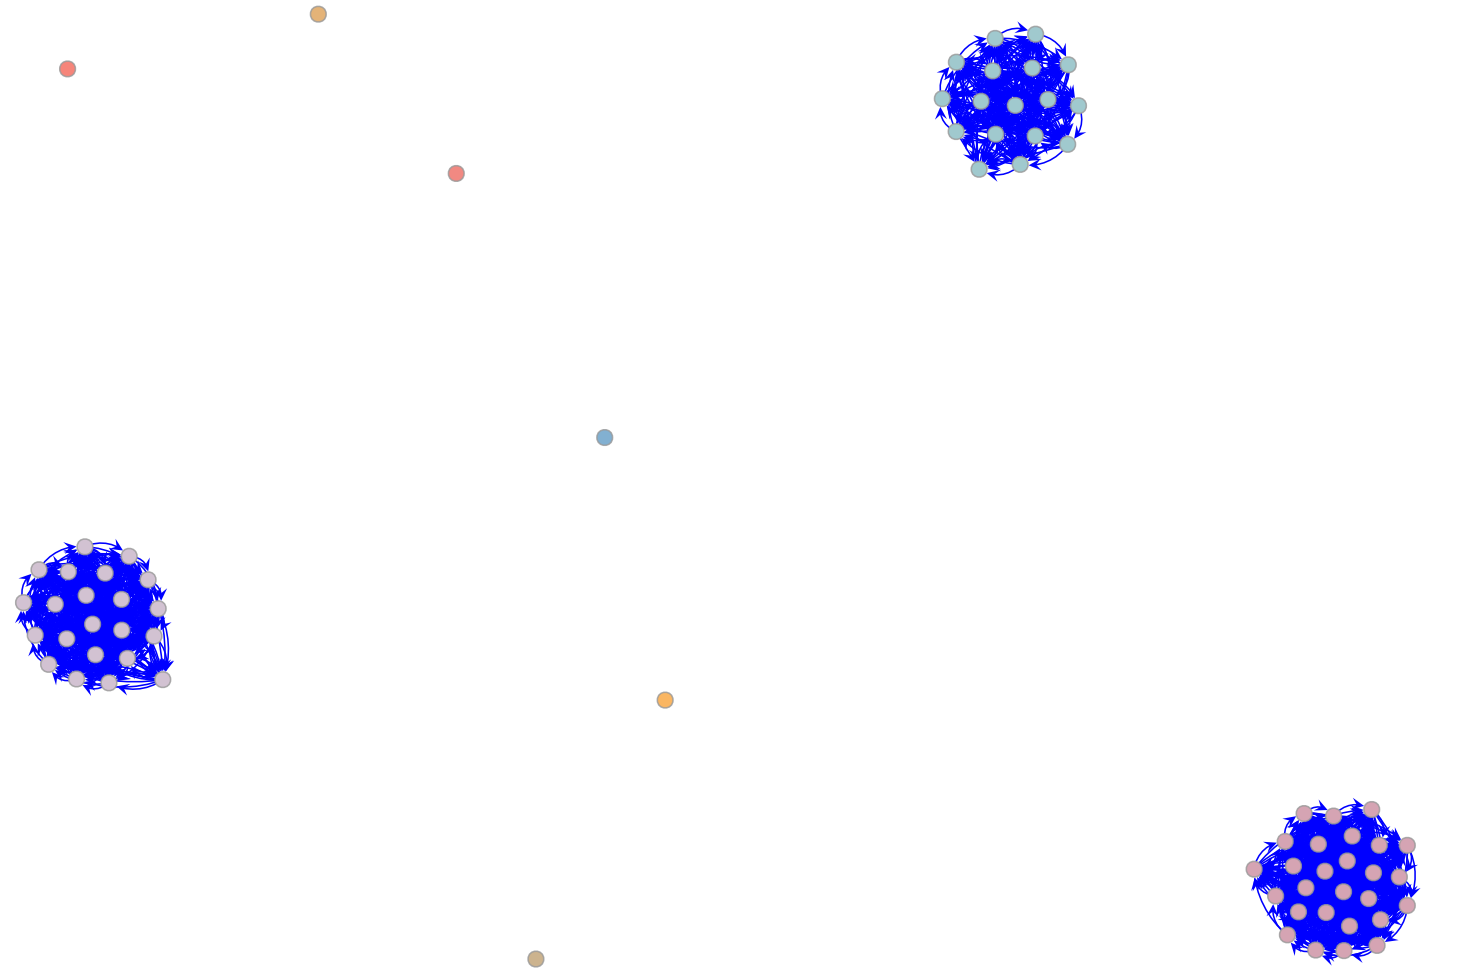
\includegraphics[width=0.95\textwidth]{bilder/all_components_5.png}
		\caption{Ausschnitt einiger Zusammenhangskomponenten des Gesamtgraphen }
		\label{fig:all_comp} 
	\end{center}
\end{figure}

Da alle weiteren Schritte des Algorithmus jeweils auf den einzelnen Komponenten durchgeführt werden, kann durch die Verwendung einer Liste von Graphen im Folgenden eine einfachen Iteration über die Komponenten ausgeführt werden, ohne dass der Filtervorgang über alle Knoten jeder Komponente wiederholt werden muss. Zudem ermöglicht diese Datenstruktur eine effizientere Traversierung und Suche innerhalb der Zusammenhangskomponente, ohne dass für jede Komponente der gesamte Graph betrachtet werden muss. Der ursprüngliche Graph wird anschließend entfernt, um Arbeitsspeicher freizugeben. \\

In der Log-Datei wird die Anzahl der Knoten aller Zusammenhangskomponenten als Histogramm festgehalten. Ebenso wird dort für alle Komponenten mit mehr als einem Element die Anzahl ihrer Knoten, Kanten und Eigenschaften aufgelistet.\\

Über die Konfigurationsdatei und die Snakemake-Regel \lstinline|noderad| können optional auch für die Zusammenhangskomponenten jeweils Visualisierungen (siehe \autoref{fig:comp}) und detaillierte Graphinformationen in den oben genannten Formaten des Graphen (Kap. \ref{subsec:edges}) ausgegeben werden. \\
\begin{figure}[H]
	\subfigure{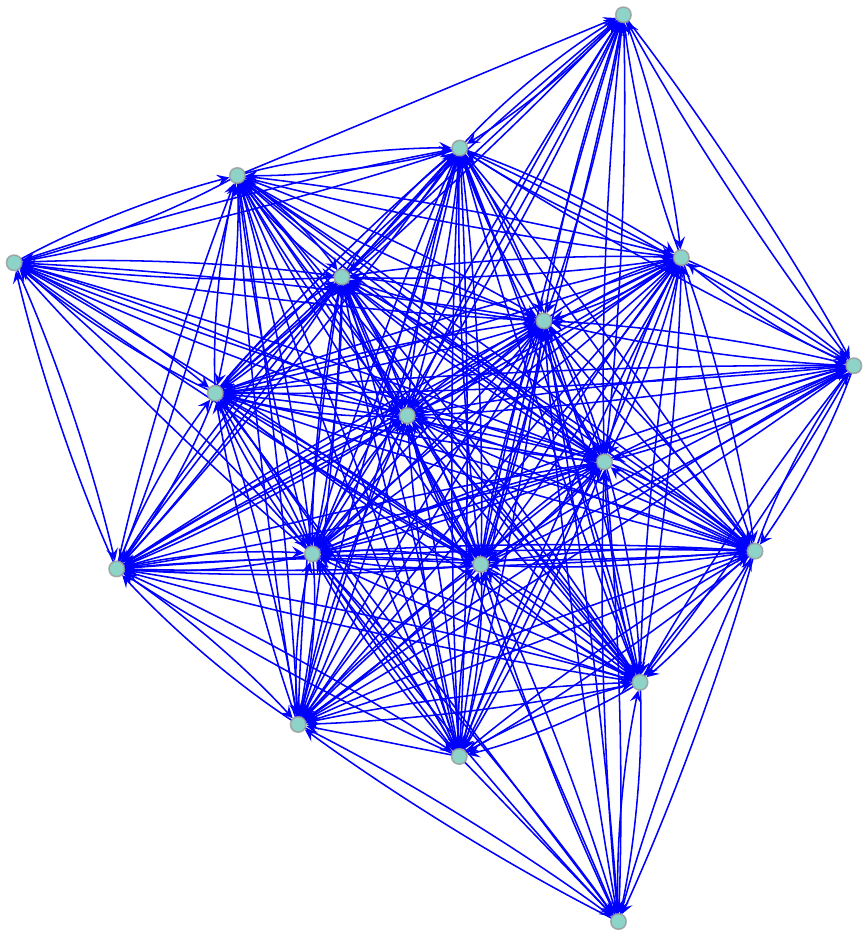
\includegraphics[width=0.22\textwidth]{bilder/small_components_2.png}}
	\subfigure{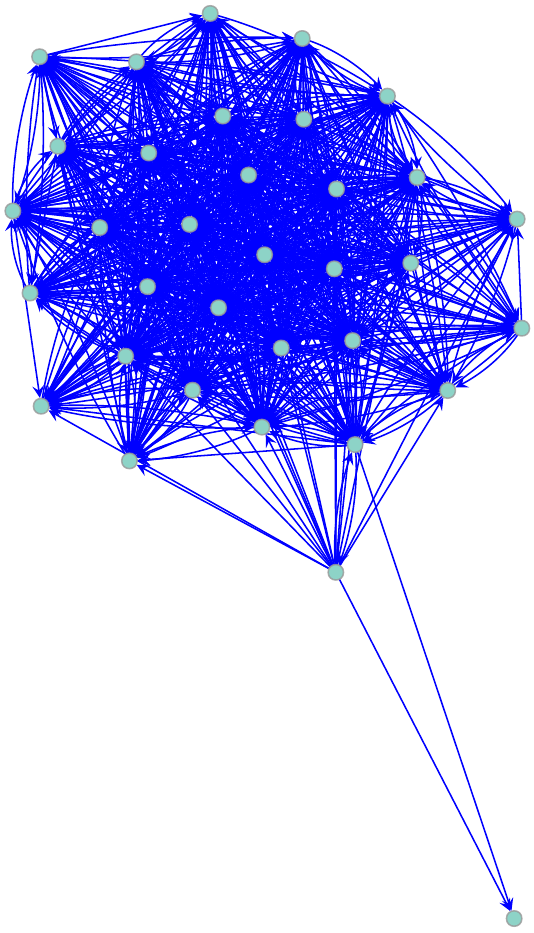
\includegraphics[width=0.25\textwidth]{bilder/medium_components_1.png}}
	\subfigure{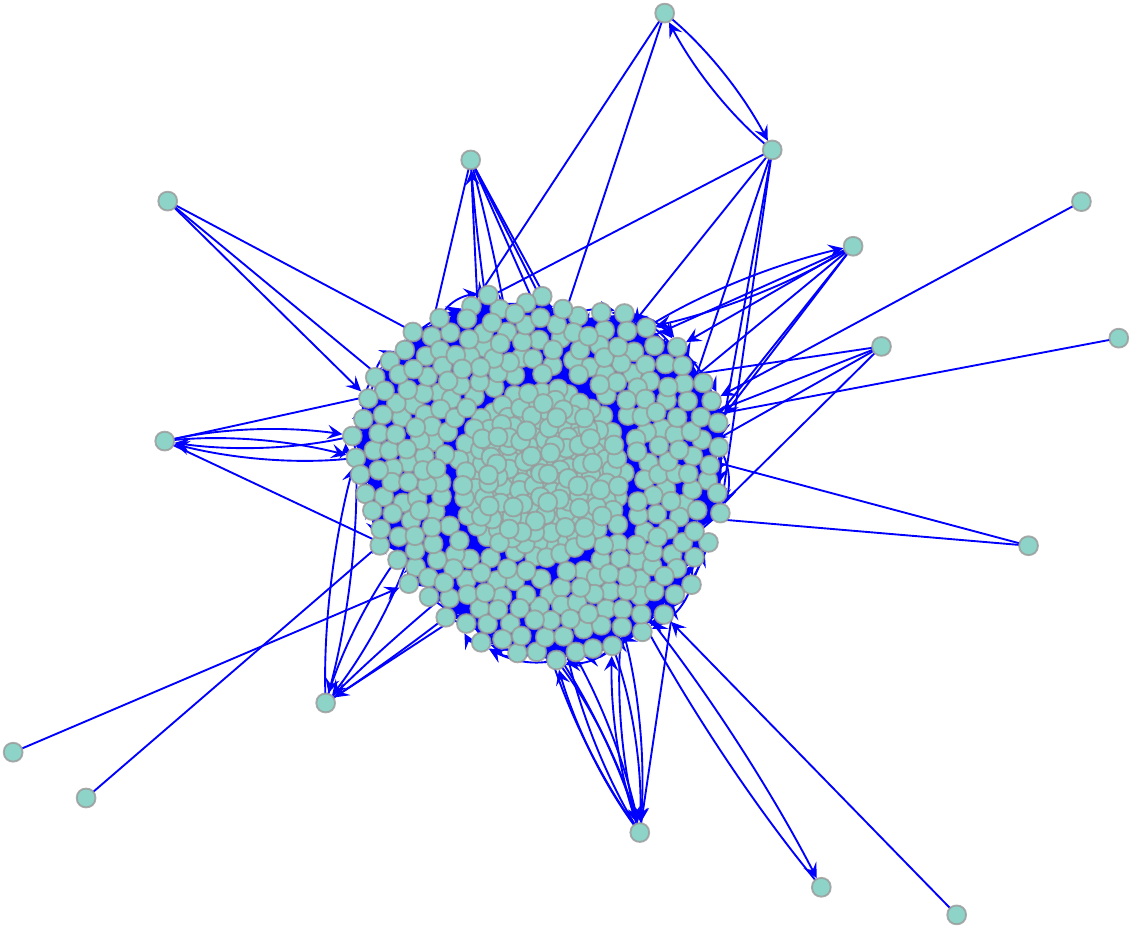
\includegraphics[width=0.50\textwidth]{bilder/big_components_2.png}}
	\caption{Beispiele von einzelnen Zusammenhangskomponenten unterschiedlicher Größe}
	\label{fig:comp}
\end{figure}

Zudem kann optional auch der gesamte Graph mit den Komponentenindizes als Knoteneigenschaften gespeichert werden. In der visuellen Darstellung werden dort seine Knoten entsprechend der zugehörigen Zusammenhangskomponente eingefärbt (siehe \autoref{fig:all_comp}).

\section{Bestimmung der Allele-Fractions mit maximaler Likelihood} \label{sec:max_lh_allele}
\subsection{Bestimmung der Kandidatenallele und ihrer möglichen Häufigkeitsverteilung} \label{subsec:cand_allele}
\begin{figure}[h]
	\begin{center}
		\begin{tikzpicture}[scale=0.63,transform shape]	
			\path (p4.south)+(0.0,-1.5) \ioitem{6}{5. Connected components};
			\path (p6.south)+(-5.5,-1.4) \blockitem{7}{\hyperref[schritt7txt]{\color{green!40} ..}7.\phantomsection\label{schritt7} Allele \\combinations};
			\path (p6.south)+(0.0,-1.4) \blockitem{8}{\hyperref[schritt6txt]{\color{green!40}..}6.\phantomsection\label{schritt6} Candidate \\alleles};			
			\path (p7.south)+(0.0,-3.9) \blockitem{9}{\hyperref[schritt8txt]{\color{green!40}..}8.\phantomsection\label{schritt8} Allele fractions};
			\path (p8.south)+(0.0,-1.5)	\ioitem{10}{9. Likelihood of alleles given one read};
			\path (p10.south)+(0.0,-1.5) \ioitem{12}{10. Likelihood of allele fractions given one read};
			\path (p12.south)+(0.0,-1.5) \ioitem{14}{11. Likelihood of allele fractions given all reads};
			\path (p14.south)+(0.0,-1.5) \ioitem{15}{12. Maximum likelihood allele fractions};
			\path (p15.south)+(0.0,-2.0) \ioitem{16}{15. Likelihood \\of an allele given another allele};			
			% Pfeile
			\path [line] (p6.south) -- node [above] {} (p8);
			\path [line] (p8.south) -- node [above] {} (p10) ;	
			\path [line] (p10.south) -- node [above] {} (p12) ;	
			\path [line] (p12.south) -- node [above] {} (p14) ;		
			\path [line] (p14.south) -- node [above, midway] {} (p15);
			\path [line] (p15.south) -- node [above] {} (p16) ;   
			
			\path (p8.east)+(+4.4, 0.0) node (ur1)[ur] {\color{black}\lstinline|get_candidate_alleles()|};
			\path (p7.east)+(-1.92,2.2) node (ur2)[ur] {\color{black}\lstinline|get_max_parsimony_n_alleles()|};
			\path (p9.east)+(-8.2,0.0) node (ur3)[ur] {\color{black}\lstinline|get_candidate_vafs()|};
		
			\path [dashedline] (p8.west) -- node [left] {} (p7);
			\path [dashedline] (p7.south) -- node [above] {} (p9) ;
			\path [dashedline] (p9.east) -- node [left] {} (p12.west);
			
			\draw [funtool] (p8.east) -- (ur1);
			\draw [funtool] (p7.north) -- (ur2);
			\draw [funtool] (p9.west) -- (ur3);
			
			\background{p2}{p8}{p4}{p15}{Allele Likelihood}
		\end{tikzpicture}
		\caption{Prozesse des Workflows - Kandidatenallele und Allele-Fractions \cite{tikz_schema}}
		\label{fig:workflow_all}
	\end{center}
\end{figure}

Die einzelnen Zusammenhangskomponenten repräsentieren einen oder mehrere Loci. Alle weiteren Berechnungen aus diesem und den folgenden Kapiteln ~\ref{sec:max_lh_loci} und ~\ref{sec:vcf} werden für jede Komponente einzeln durchgeführt, dabei sollen die wahrscheinlichsten Allelsequenzen und die dazugehörigen Loci identifiziert werden. Alle hierfür implementierten Funktionen finden sich im Modul \lstinline|likelihood_operations.py|. \\

Zunächst werden mit der Funktion \hyperref[schritt6]{\lstinline|get_candidate_alleles()|\phantomsection\label{schritt6txt}} die Allelsequenzen ermittelt, die in der Zusammenhangskomponenten vorkommen und deren Häufigkeiten bestimmt. Übersteigt die Größe eines Clusters, d.h. die Knotenanzahl einer Zusammenhangskomponenten, den in der Konfigurationsdatei unter \lstinline|treshold-seq-noise| festgelegten Grenzwert \lstinline|large-clusters|, so werden nur diejenigen Sequenzen als Kandidatenallele ausgewählt, deren Häufigkeit über dem \lstinline|large-clusters| Schwellenwert liegt. Dies dient dazu, bei großen Clustern Komplexität und Rechenaufwand zu reduzieren, da davon auszugehen ist, dass innerhalb eines großen Clusters echte Varianten einer Sequenz mehrfach vorkommen, wohingegen Artefakte und Sequenzierfehler eher vereinzelt auftreten. Dieses sog. Rauschen kann durch Anpassung der Schwellwerte in der Konfigurationsdatei herausgefiltert werden. Ebenso kann es jedoch vorkommen, dass auch bei kleinen Clustern viele verschiedene Sequenzen auftreten, so dass es durch eine hohe Anzahl von Kandidatenallele zu einem erheblichen Rechenaufwand bei der späteren Analyse kommen kann. Um dem entgegenwirken, kann durch einen weiteren unter \lstinline|treshold-seq-noise| festgelegten Grenzwert \lstinline|small-clusters| die Mindesthäufigkeit der Sequenzen bei kleineren Clustern unterhalb von \lstinline|treshold-cluster-size| angegeben werden. Da bei kleinen Clustern auch einmalig registrierte Varianten einer Sequenz von Bedeutung sein können, sollte der Filtervorgang hier möglichst gering gehalten werden. Gilt \lstinline|small-clusters = 1|, so wird die Option für kleine Cluster vollständig deaktiviert. \\

Die Kandidatenallele werden anschließend für deterministischere Ergebnisse lexikographisch sortiert und als Liste $ A_{cand} $ der Länge $ n_{cand} $ von \lstinline|get_candidate_alleles()| zurückgegeben. Aus dieser Liste sollen nun die möglichen Häufigkeitsverteilungen in Abhängigkeit von der Ploidie bestimmt werden. Hierzu muss zunächst die aufgrund der Ploidie tatsächlich zu erwartende Anzahl von Allelen $n_{alleles}$ bestimmt werden. Dies geschieht durch die Funktion \hyperref[schritt7]{\lstinline|get_max_parsimony_n_alleles()|\phantomsection\label{schritt7txt}}. Dadurch werden unnötige bzw. nicht mögliche Allelkombinationen eingespart und in der weiteren Berechnung nicht berücksichtigt. Ist die Ploidie $ \phi $ höher als die Anzahl der Kandidatenallele, so muss es mindestens genauso viele und bei Homozygotie auch mehrfach vorkommende Allele geben, damit die Ploidie erfüllt werden kann. Es muss also gelten $ n_{alleles} = \phi $. Wurden dagegen mehr Allele beobachtet als aufgrund der Ploidie möglich sind und die Ploidie ist Teiler von $n_{cand}$, so können alle beobachteten Allele auch tatsächlich vorkommen, da die Zusammenhangskomponente auch mehrere Loci enthalten kann. Es gilt dann also $ n_{alleles} = n_{cand} $. Ist dagegen die Anzahl der beobachteten Allele höher als die Ploidie, aber nicht ganzzahlig durch die Ploidie teilbar, so muss die Anzahl der Allele entsprechend erhöht werden. Das heißt, es müssen tatsächlich so viele Allele vorkommen, dass eine korrekte Ploidie erreicht wird, dass also die Ploidie eine Teiler von $ n_{alleles} $ wird. Die Anzahl der Allele muss also um die Ploidie abzüglich des Restes aus der Restdivision erhöht werden und es gilt $ n_{alleles} = n_{cand} + \phi - (n_{cand} \mod \phi)$. \\

Mit Hilfe der tatsächlich zu erwarteten Anzahl von Allelen $ n_{alleles} $ können nun alle Kombinationen möglicher Häufigkeitsverteilungen der Allele bestimmt werden (Funktion \hyperref[schritt8]{\lstinline|get_candidate_vafs()|\phantomsection\label{schritt8txt}}). Diese Häufigkeitsverteilungen werden auch als Allele-Fractions bezeichnet. Hierfür werden zunächst alle möglichen Allelkombinationen ermittelt. Dies erfolgt nach dem Urnenmodell unter Auswahl von $ n_{alleles} $ Elementen mit Zurücklegen aus insgesamt $ n_{cand} $ verschiedenen Elementen und ohne Berücksichtigung der Reihenfolge. Dadurch berechnet sich die Anzahl möglicher Kombination nach \eqref{eqn:3-1} aus dem  Binomialkoeffizienten der $k$-ten Ordnung aus $ n $ Elementen mit Zurücklegen ~\cite{tb_stat,bronst}.
\begin{equation} \label{eqn:3-1}
\tag{3-1}
\binom{n + k - 1}{k} = \frac{(n+k-1)!}{(n-1)!\, \cdotp k!} = \frac{(n_{alleles}+n_{cand}-1)!}{(n_{alleles}-1)!\, \cdotp n_{cand}!} 
\end{equation}

Die Allelkombinationen werden mit Hilfe der Funktion  \lstinline|combinations_with_replacement| aus der Python-Library \lstinline|itertools| erzeugt \cite{itertools}.\\
\\
\fcolorbox{black}{light-gray}{
	\parbox{\textwidth}{
		\vspace{0.5cm}
		\textbf{Beispiele möglicher Allelkombinationen:} \\	
		\\	
		$ ploidy = 2, n_{cand} = 2, n_{alleles} = 2$: \\
		{[(0, 0), (0, 1), (1, 1)]}\\
		\\
		$ ploidy = 2, n_{cand} = 3, n_{alleles} = 4$: \\
		{[(0, 0, 0, 0), (0, 0, 0, 1), (0, 0, 0, 2), (0, 0, 1, 1), (0, 0, 1, 2), (0, 0, 2, 2), (0, 1, 1, 1), (0, 1, 1, 2), (0, 1, 2, 2), (0, 2, 2, 2), (1, 1, 1, 1), (1, 1, 1, 2), (1, 1, 2, 2), (1, 2, 2, 2), (2, 2, 2, 2)]}
		\\
	}}\\


Für jedes Allel $a_{i}$ können im Anschluss aus seinen absoluten Häufigkeiten $H_{a_{i}}$ innerhalb jeder Allelkombination die relativen Häufigkeiten $h_{a_{i}}$ nach \eqref{eqn:3-2} bestimmt werden. 
\begin{equation} \label{eqn:3-2}
\tag{3-2}
h_{a_{i}} = \frac{H_{a_{i}}} {n_{alleles}}
\end{equation}

\begin{center}	
\fcolorbox{black}{light-gray}{
	\parbox{\textwidth}{
		\vspace{0.5cm}
		\textbf{Beispiele möglicher Allele-Fractions:} \\	
		\\	
		$ ploidy = 2, n_{cand} = 2, n_{alleles} = 2$: \\
		{[1.0, 0.0]}, {[0.5, 0.5]}, {[0.0, 1.0]} \\
		\\
		$ ploidy = 2, n_{cand} = 3, n_{alleles} = 4$: \\
		{[1.0, 0.0, 0.0]}, {[0.75, 0.25, 0.0]}, {[0.75, 0.0, 0.25]}, {[0.5, 0.5, 0.0]}, {[0.5, 0.25, 0.25]}, {[0.5, 0.0, 0.5]}, {[0.25, 0.75, 0.0]}, {[0.25, 0.5, 0.25]}, {[0.25, 0.25, 0.5]}, {[0.25, 0.0, 0.75]}, {[0.0, 1.0, 0.0]}, {[0.0, 0.75, 0.25]}, {[0.0, 0.5, 0.5]}, {[0.0, 0.25, 0.75]}, {[0.0, 0.0, 1.0]}
		\\
}}
\end{center}

\subsection{Berechnung der Likelihoods der Allele anhand der Allele-Fractions} \label{subsec:lh_allele}
\begin{figure}[h]
	\begin{center}
		\begin{tikzpicture}[scale=0.63,transform shape]	
		\path (p4.south)+(0.0,-1.5) \ioitem{6}{5. Connected components};
		\path (p6.south)+(-5.5,-1.4) \ioitem{7}{7. Allele \\combinations};
		\path (p6.south)+(0.0,-1.4) \ioitem{8}{6. Candidate \\alleles};			
		\path (p7.south)+(0.0,-3.9) \ioitem{9}{8. Allele fractions};
		\path (p8.south)+(0.0,-1.5)	\blockitem{10}{\hyperref[schritt9txt]{\color{green!40}..}9.\phantomsection\label{schritt9} Likelihood of alleles given one read};
		\path (p10.south)+(0.0,-1.5) \blockitem{12}{\hyperref[schritt10txt]{\color{green!40}.\color{black}1}0.\phantomsection\label{schritt10} Likelihood of allele fractions given one read};
		\path (p12.south)+(0.0,-1.5) \blockitem{14}{\hyperref[schritt11txt]{\color{green!40}.\color{black}1}1.\phantomsection\label{schritt11} Likelihood of allele fractions given all reads};
		\path (p14.south)+(0.0,-1.5) \blockitem{15}{\hyperref[schritt12txt]{\color{green!40}.\color{black}1}2.\phantomsection\label{schritt12} Maximum likelihood allele fractions};
		\path (p15.south)+(0.0,-2.0) \ioitem{16}{15. Likelihood \\of an allele given another allele};
		\path (p10.east)+(+4.1,0.0) node (ur1)[ur] {\color{black}\lstinline|get_allele_likelihood_read()|};
		\path (ur1.east)+(-2.915,2.1) node (ur2)[ur] {\color{black}\lstinline|get_alignment_likelihood()|};
		\path (p12.east)+(8.0-4,0) node (ur3)[ur] {\color{black}\lstinline|calc_vafs_likelihood_read()|};
		\path (p14.east)+(9.5-6,0) node (ur4)[ur] {\color{black}\lstinline|calc_vafs_likelihood()|};
		
		% Pfeile
		\path [line] (p6.south) -- node [above] {} (p8);
		\path [line] (p8.south) -- node [above] {} (p10) ;	
		\path [line] (p10.south) -- node [above] {} (p12) ;	
		\path [line] (p12.south) -- node [above] {} (p14) ;		
		\path [line] (p14.south) -- node [above, midway] {} (p15);
		\path [line] (p15.south) -- node [above] {} (p16) ;   
		
		\path [dashedline] (p8.west) -- node [left] {} (p7);
		\path [dashedline] (p7.south) -- node [above] {} (p9) ;
		\path [dashedline] (p9.east) -- node [left] {} (p12.west);
		
		\draw [funtool] (p10.east) -- (ur1);
		\draw [dashedline] (ur2.south) -- (ur1.north);
		\draw [funtool] (p12.east) -- (ur3);
		\draw [funtool] (p14.east) -- (ur4);
		
		\background{p2}{p8}{p4}{p15}{Allele Likelihood}
		\end{tikzpicture}
		\caption{Prozesse des Workflows - Likelihood der Allele-Fractions \cite{tikz_schema}}
		\label{fig:workflow_all}
	\end{center}
\end{figure}
In diesem Kapitel soll diejenige Allel-Fraction bestimmt werden, welche die beobachteten Reads am besten erklärt (vgl. Kap. \ref{subsec:sol_allele_lh}). Für jeden Read wird dafür zunächst die Wahrscheinlichkeit bestimmt, dass der Read durch Sequenzierfehler aus einem der Kandidatenallele entstanden ist. Hiernach wird für jeden Read die Wahrscheinlichkeit errechnet, diesen anhand einer gegebenen Allele-Fraction zu beobachten. Diese Berechnungen werden für alle Allele-Fractions durchgeführt. Aus der so gewonnenen Lösungsmenge wird die Allel-Fraction mit der höchsten Likelihood für die spätere Zuordnung der Loci (Kap. \ref{sec:max_lh_loci}) ausgewählt. \\ 

Zunächst wird in der Funktion \hyperref[schritt9]{\lstinline|get_allele_likelihood_read()|\phantomsection\label{schritt9txt}} eine Kante zwischen dem betrachteten Read und dem Kandidatenallel gesucht. Während der Ausführung werden die Sequenzen und Likelihoods der bereits gefundenen Read-Kandidatenallel-Paare in einem Dictionary abgelegt. Als Key wird dabei das Tupel aus der Read-ID und der Allelsequenz verwendet, die berechnete Likelihood wird als Value eingetragen. Da später für die Likelihoodberechnungen der verschiedenen Allel-Fraktions mehrfach die Werte der Read-Allel-Likelihoods verwendet werden, ermöglicht die Verwendung eines Dictionary eine schnellere und effizientere Suche der passenden Kante ohne wiederholte Likelihoodberechnung. \\

Existiert für ein Read-Kandidatenallel-Paar noch kein Eintrag im Dictionary, so werden zuerst alle ausgehenden Nachbarn des Reads hinsichtlich ihrer in den Knoteneigenschaften abgelegten Sequenz geprüft. Besitzt einer der ausgehenden Nachbarknoten die Sequenz des Kandidatenallels, so wird die Likelihood durch \lstinline|get_alignment_likelihood()| berechnet (Algorithmus \ref{alg:lh_read}), ein entsprechender Eintrag im Dictionary angelegt und die Likelihood zurückgegeben.\\

Gibt es keine solche Kante, die vom Read zu einem Knoten mit Kandidatenallelsequenz führt, so wird geprüft, ob es eine Kante in umgekehrter Richtung gibt. Hierfür werden nun alle eingehenden Nachbarn des Reads betrachtet. Findet sich unter ihnen ein Knoten mit der gesuchten Kandidatenallelsequenz, so wird mit \lstinline|get_alignment_likelihood()| die Likelihood berechnet, wobei die Verwendung der Gegenrichtung durch das Argument \lstinline|reverse=True| markiert wird. Existiert auch keine entgegengesetzt gerichteten Kante, so wird der Wert $0$ zurückgegeben.\\

Zur Veranschaulichung ist der beschriebene Algorithmus zudem in Pseudocode dargestellt (Algorithmus \ref{alg:r-a-lh}). Dabei sind $ C_{k} \in \{C_{1}, \dots ,C_{p}\} $ der Subgraph einer Zusammenhangskomponente, $ r_{i} \in C_{k} $ der Knoten des Reads mit der ID $ idx_{r_{i}}$ und $ a_{j} \in A_{cand} $ ein Kandidatenallel mit der Sequenz $ s_{a_{j}} $, wobei $ k,i,j \in \mathds{N} $. Das oben beschriebene Dictionary $dict$ besitzt als Keys die Tupel der Sequenzen $(idx_{r_{i}}, s_{a_{i}}) $ und als Values die Likelihoods $L_{r_{i}, a_{i}}$, so dass gilt $ ((idx_{r_{i}}, s_{a_{i}}), L_{r_{i}, a_{i}})  \in dict $. Die Verwendung fester Knoten- oder Kanteneigenschaften ist durch eckige Klammern gekennzeichnet, so ruft beispielsweise $r_{i}[q\_values]$ die $ q $-Werte des Phred Quality Scores von $r_{i}$ auf.\\

\renewcommand{\algorithmiccomment}[1]{\hfill$\triangleright$\textit{#1}}
\begin{algorithm}[H]
	\caption{Suche eines Alignments zwischen Read und Kandidatenallel} \label{alg:r-a-lh}
	\begin{algorithmic}[1]	
		\Function{get\_allele\_likelihood\_read}{$ C_{k} $, $ r_{i} $, $ s_{a_{j}} $, $ dict $}
		\State $ idx_{r_{i}} \gets r_{i}[name]$
		\State $ qual \gets r_{i}[q\_values] $
		\State $ \epsilon \gets C_{k}[\epsilon_{ins}] \cup C_{k}[\epsilon_{del}] $
		\If{$\exists (idx_{r_{i}}, s_{a_{i}}): ((idx_{r_{i}}, s_{a_{i}}), L_{r_{i}, a_{i}}) \in dict$}
		\State \Return $ L_{r_{i}, a_{i}} $
		\EndIf		
		\State $ out\_neighbors \gets get\_out\_neighbors(r_{i})$
		\For {$out\_neighbor \in out\_neighbors $}
		\If{$ s_{a_{j}} = out\_neighbor[sequence] $}
		\State $ cig \gets edge(r_{i}, out\_neighbor)[cigar\_tuples]$		
		\State $ rev \gets False $
		\State $ L_{r_{i}, a_{i}} \gets get\_alignment\_likelihood(\epsilon,\, cig,\, qual,\, rev)$
		\algorithmiccomment{Alg. \ref{alg:lh_read}}
		\State $ dict \gets dict \, \cup ((r_{i}, out\_neighbor[sequence]), L_{r_{i}, a_{i}})  $
		\State \Return $L_{r_{i}, a_{i}}$   
		\EndIf
		\EndFor		
		\State $ in\_neighbors \gets get\_in\_neighbors(r_{i})$		
		\For {$in\_neighbor \in in\_neighbors $}
		\If{$ s_{a_{j}} =  in\_neighbor[sequence] $}		
		\State $ cig \gets edge(in\_neighbor, r_{i})[cigar\_tuples]$		
		\State $ rev \gets True $
		\State $ L_{r_{i}, a_{i}} \gets get\_alignment\_likelihood(\epsilon,\, cig,\, qual,\, rev)$
		\algorithmiccomment{Alg. \ref{alg:lh_read}}
		\State $ dict \gets dict \, \cup ((r_{i}, in\_neighbor[sequence]), L_{r_{i}, a_{i}})  $
		\State \Return $L_{r_{i}, a_{i}}$  
		\EndIf		
		\EndFor		
		\State \Return 0
		\EndFunction
	\end{algorithmic}
\end{algorithm}

Die eigentliche Likelihoodberechnung erfolgt in der Methode \linebreak \lstinline|get_alignment_likelihood()| (Algorithmus \ref{alg:lh_read}) nach Formel \eqref{eqn:2-9} des Modells. Wie in Kap. \ref{subsec:phmm_minimap} beschrieben wird hierfür die Approximation des PairHMM aus den Sequenzalignments von Minimap2 verwendet.\\

Von der in \lstinline|get_allele_likelihood_read()| ermittelten Kante zwischen Read und Kandidatenallel werden der Funktion die CIGAR-Tupel aus den Kanteneigenschaften, der Vektor mit dem  Phred Quality Scores $Q =(q_{1}, \dots, q_{m})$ aus den Knoteneigenschaften des Reads (siehe Kap. \ref {subsec:nodes}) sowie die Kantenrichtung als boolescher Wert übergeben. Aus den Phred Quality Scores des Reads wird zunächst die geschätzte Fehlerwahrscheinlichkeit $ P=(p_{1}, \dots, p_{m}) $ für jede Base nach Formel \eqref{eqn:3-3} errechnet ~\cite{ewing_1998}.  
\begin{equation} \label{eqn:3-3}
\tag{3-3}
p_{i} = 10^{\frac{-q_{i}}{10}}
\end{equation}

Im Anschluss wird aus den p-Werten der Basenqualität für jede Base des Reads die Wahrscheinlichkeit errechnet, dass es sich im Falle eines Matches um die korrekte Base handelt \eqref{eqn:2-6} bzw. im Falle eines Mismatches, dass sich der Read durch Sequenzierfehler aus dem Allel erklären lässt \eqref{eqn:2-3}. Für Indels werden die empirisch ermittelten Sequenzierfehlerraten von Illumina für Sequenzierplattformen~\cite{schirmer_2016} aus der Konfigurationsdatei unter dem Parameter \lstinline|errors-per-base| entnommen. Entsprechend den in den CIGAR-Tupeln angegebenen Operationen wird für jede Base die Likelihood berechnet. Das Produkt der Likelihoods der einzelnen Basen ergibt schließlich die Likelihood zwischen Read und Allel \eqref{eqn:2-4}.\\

Bei Bedarf kann die Methode \lstinline|get_alignment_likelihood()| auch  die Likelihood der entgegengesetzt gerichteten Kante bestimmen. Dabei wird die Querysequenz als Referenzsequenz betrachtet und umgekehrt. Dies ist über das boolesche Argument \lstinline|reverse| steuerbar. Gilt \lstinline|reverse = True|, so werden für die übergebenen CIGAR-Tupel Insertionen zu Deletionen und Deletionen zu Insertionen umgewandelt.\\

Zur Veranschaulichung ist die Methode in Algorithmus \ref{alg:lh_read} zusätzlich als Pseudocode verfasst. Die Wahrscheinlichkeiten für Sequenzierfehler bei Insertionen und Deletionen aus den Grapheigenschaften werden dort mit $ \epsilon_{ins} $ und $ \epsilon_{del} $ bezeichnet, der Vektor der Phred Quality Scores der Querysequenz mit $q_{query}$
\newpage
\begin{algorithm}[H]
	\caption{Berechnung der Likelihood zwischen Read und Kandidatenallel}  \label{alg:lh_read}
	\begin{algorithmic}[1]	
		\Function{get\_alignment\_likelihood}{$ \epsilon_{ins} $, $ \epsilon_{del} $, $ cigar\_tuples $, $ q_{query} $, reverse}
		\State $ likelihood \gets 1.0 $, $ index \gets 0 $, $ p_{query} \gets [\;] $
		\For{$ q_{i} \in q_{query} $}
		\State $p_{query} \gets p_{query}\, \cup \, (10^{\frac{-q_{i}}{10}}) $
		\EndFor			
		\If {$reverse$}
		\State swap values of $ \epsilon_{ins} $ and $ \epsilon_{del} $
		\EndIf
		\ForAll {$ (operation, length) \in cigar\_tuples $}
		\While{$ index < (index + length) $}		
		\If {$operation \in match $}		
		\State $ likelihood\, \gets likelihood \,\cdotp (1-p_{query}[index]) $
		\EndIf
		\If {$operation \in substitution $}
		\State $ likelihood\, \gets likelihood \,\cdotp \frac{1}{3} \,\cdotp p_{query}[index] $
		\EndIf
		\If {$operation \in insertion $}
		\State $ likelihood\, \gets likelihood \,\cdotp \epsilon_{ins}$
		\EndIf
		\If {$operation \in deletion $}
		\State $ likelihood\, \gets likelihood \,\cdotp \epsilon_{del} $
		\EndIf
		\State $index \gets index + 1 $
		\EndWhile
		\EndFor
		\State \Return $likelihood$
		\EndFunction		
	\end{algorithmic}
\end{algorithm}

Durch \lstinline|get_allele_likelihood_read()| und \lstinline|get_alignment_likelihood()| wurden also die Wahrscheinlichkeiten jedes Reads bestimmt, dass er von den verschiedenen Allelen der Zusammenhangskomponente stammt (siehe oben). Die Wahrscheinlichkeiten im Bezug auf jedes Allel sollen nun in die zuvor bestimmten Allele-Fractions (siehe Kap. \ref{subsec:cand_allele}) nach Formel \eqref{eqn:2-10} einbezogen werden. In der Funktion \hyperref[schritt10]{\lstinline|calc_vafs_likelihood_read()|\phantomsection\label{schritt10txt}} wird nun für jeden Read die Wahrscheinlichkeit berechnet, diesen unter der gegebenen Allel-Fraction zu beobachten. Dazu wird über die relativen Häufigkeiten jedes Allels der Allele-Fraction iteriert und ihr Produkt mit der Readlikelihood aufsummiert. \\

Aus dem Produkt über alle Reads wird anschließend für die Allele-Fraction nach Formel \eqref{eqn:2-11} in \hyperref[schritt11]{\lstinline|calc_vafs_likelihood()|\phantomsection\label{schritt11txt}} die Gesamtwahrscheinlichkeit errechnet. \\

Auf diese Weise wird in \lstinline|noderad_main.py| für jede Allel-Fraction die Gesamtwahrscheinlichkeit über alle Reads und alle relativen Häufigkeiten der Allele berechnet und in einer Liste abgelegt. \\

Aus dieser Liste wird die Allele-Fraction mit \hyperref[schritt12]{maximaler Likelihood\phantomsection\label{schritt12txt}} als wahrscheinlichste Lösung gewählt und in Kap. \ref{sec:max_lh_loci} verwendet, um die wahrscheinlichsten Loci zu ermitteln, die diese Häufigkeitsverteilung der Allele erklären können.  \\

Als zusätzliche Statistiken werden in den Log-Dateien für jede Komponente die Anzahl der Allele, die Ploidie sowie Allele-Fraction mit der maximaler Likelihood und den dazugehörigen Allelsequenzen festgehalten.

\section{Bestimmung der maximalen Likelihood der Loci} \label{sec:max_lh_loci}

In Abhängigkeit von der Anzahl der Kandidatenallele und der Ploidie können die Zusammenhangskomponenten auch mehr als nur einen Locus beinhalten. Daher soll die in Kap. \ref{sec:max_lh_allele} identifizierte Allelfraktion mit maximaler Likelihood nun passenden Loci-Kombinationen zugeordnet werden. Unter Einbeziehung der Heterozygotiewahrscheinlichkeiten soll daraus die wahrscheinlichste Loci-Zuordnung ermittelt werden.

\subsection{Bestimmung der möglichen Loci} \label{subsec:comb_loci}

\begin{figure}[h]
	\begin{center}
		\begin{tikzpicture}[scale=0.64,transform shape]
		\path (p9.south)+(0.0,-7.58) \ioitem{11}{\hyperref[schritt14atxt]{\color{green!40}.\color{black}1}4.\phantomsection\label{schritt14a} Indicator constrait};
		\path (p11.south)+(0.0,-1.5) \blockitem{13}{\hyperref[schritt13txt]{\color{green!40}..}13.\phantomsection\label{schritt13} Loci \\combinations};
		\path (p14.south)+(0.0,-1.5) \ioitem{15}{12. Maximum likelihood allele fractions};
		\path (p15.south)+(0.0,-2.0) \ioitem{16}{15. Likelihood \\of an allele given another allele};
		\path (p16.south)+(0.0,-1.8) \ioitem{17}{16. Likelihood of loci given alleles and fractions}; 
		\path (p17.south)+(0.0,-1.3) \ioitem{18}{17. Maximum likelihood loci};
		\path (p18.south)+(0.0,-1.7) \ioitem{19}{18. VCF \\ 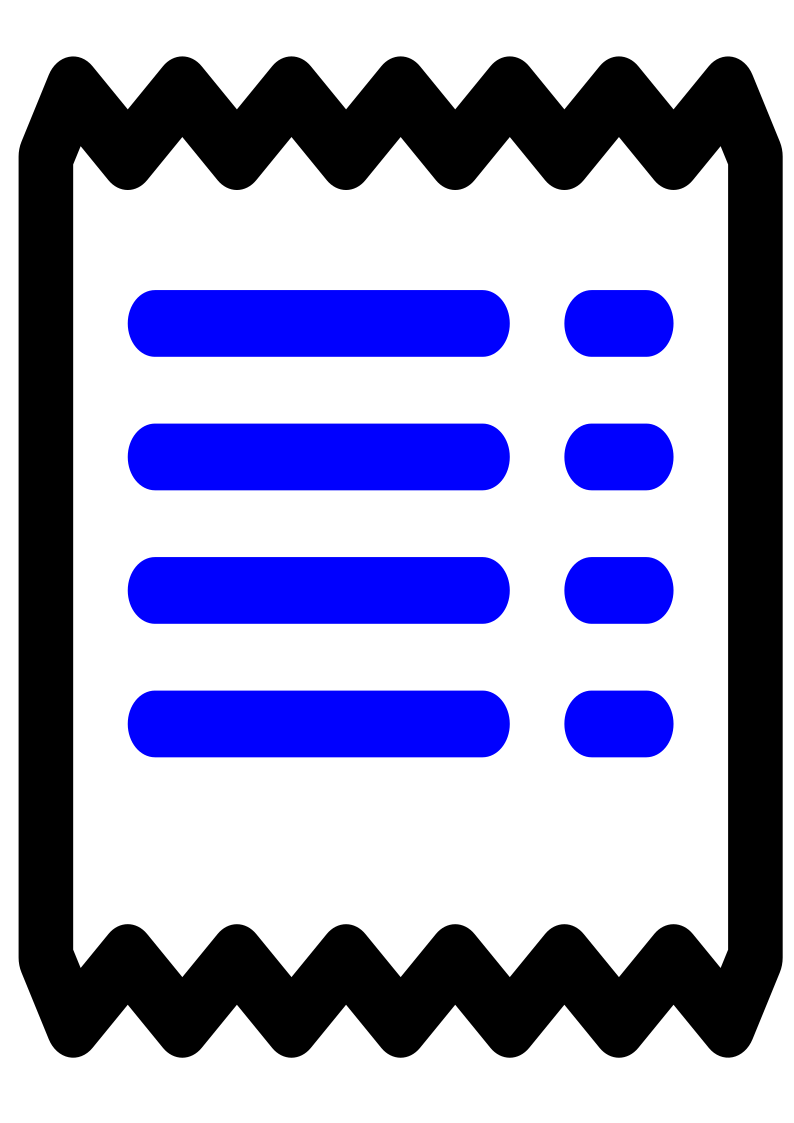
\includegraphics[width=0.9cm]{bilder/list_icon_2.png}\hspace{0.1cm}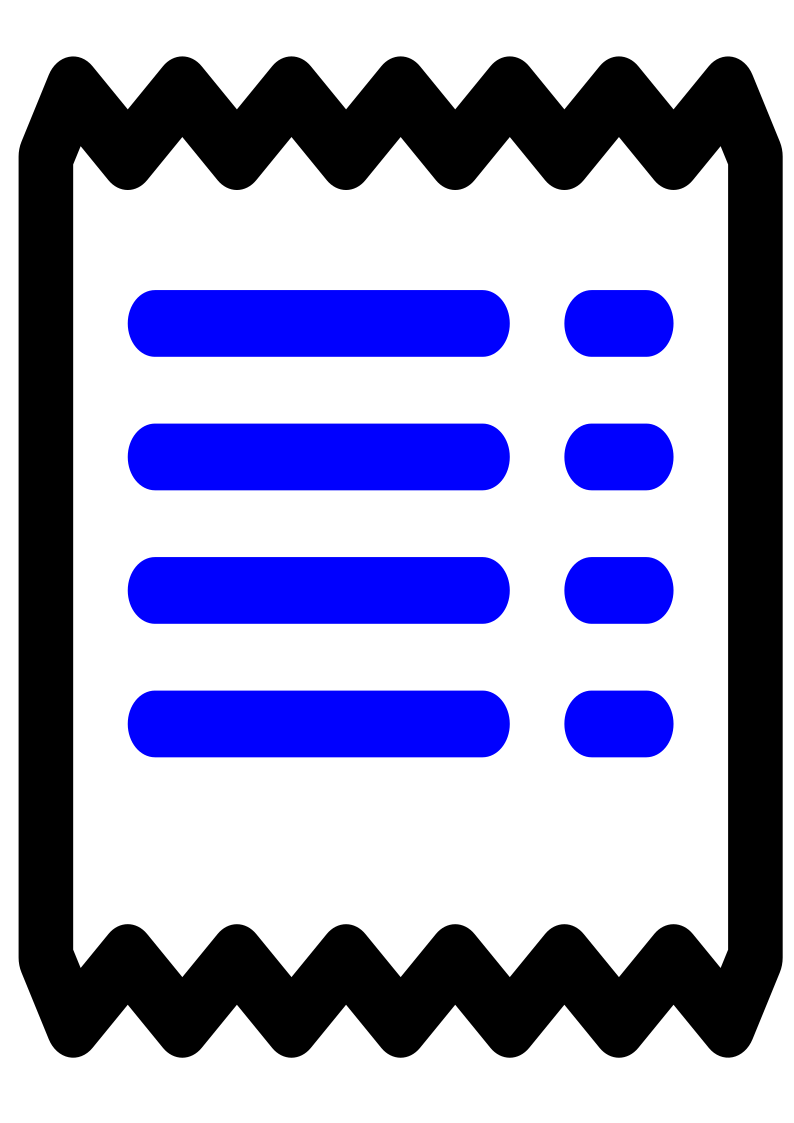
\includegraphics[width=0.9cm]{bilder/list_icon_2.png}\hspace{0.1cm}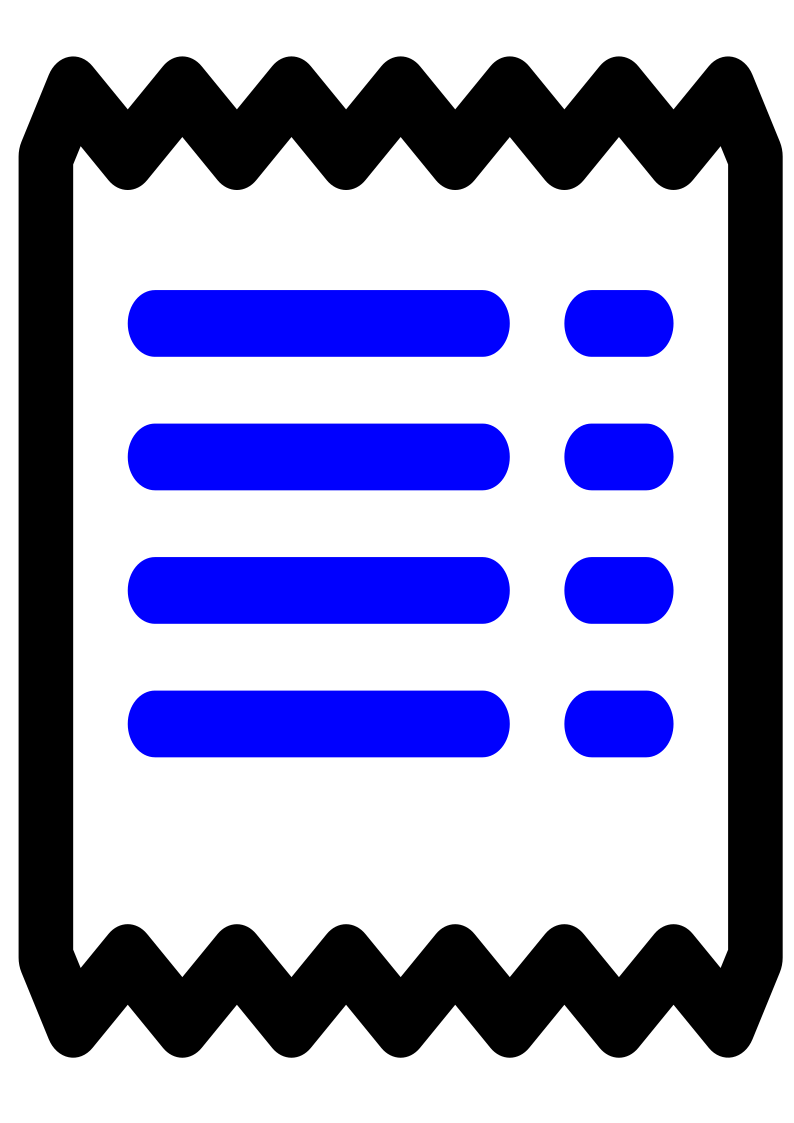
\includegraphics[width=0.9cm]{bilder/list_icon_2.png}};
		\path (p13.west)+(-4.5, 0.0) node (ur1)[ur] {\color{black}\lstinline|get_candidate_loci()|};
		% Pfeile
		\path [line] (p15.south) -- node [above] {} (p16) ;     
		\path [line] (p16.south) -- node [above] {} (p17) ;
		\path [line] (p17.south) -- node [above] {} (p18) ;
		\path [line] (p18.south) -- node [above] {} (p19) ;		
		
		\path [dashedline] (p11.east) -- node [left] {} (p16.west);
		\path [dashedline] (p13.north) -- node [left] {} (p11.south); 

		\draw [funtool] (p13.west) -- (ur1.east);

		\background{p2}{p16}{p4}{p18}{Loci Likelihood}
	\end{tikzpicture}
	\caption{Prozesse des Workflows - Loci-Kombinationen \cite{tikz_schema, bootstrap}}
	\label{fig:workflow_all}
\end{center}
\end{figure}

Für die Zuordnung der Loci müssen zunächst aus der Allele-Fraction mit maximaler Likelihood die  verschiedenen Kombinationen möglicher Loci durch \hyperref[schritt13]{\lstinline|get_candidate_loci()|\phantomsection\label{schritt13txt}} erzeugt werden. Die Funktion ist bereits in einer effizienteren Form implementiert und die zugrundeliegenden Verbindungen zum Modell sind dadurch nicht direkt erkennbar. Aus diesem Grund sollen an dieser Stelle zunächst die Überlegungen aufgezeigt werden, auf denen die effizientere Implementierung basiert, im Anschluss werden die Änderungen zur Effizienzverbesserung aufgezeigt. \\

Analog zu \lstinline|get_candidate_vafs()| (Kap. \ref{subsec:cand_allele}) sollen aus der beobachteten $n_{cand} $ und der tatsächlich zu erwartenden Anzahl von Allelen $n_{alleles}$ alle Allelkombinationen mit Wiederholung und ohne Berücksichtigung der Reihenfolge  (vgl. Formel \eqref{eqn:3-1}) durch die Funktion \lstinline|combinations_with_replacement()| aus der Python-Library \lstinline|itertools| gebildet. Allerdings sollen nun die Allelkombinationen zu Tupeln entsprechend ihrer Ploidie zusammengefasst werden. Jedes Tupel repräsentiert einen möglichen Locus in der Kombination. Die Allelkombinationen durch \lstinline|combinations_with_replacement()| sind lexikographisch sortiert. Für jede der Kombinationen muss nun aber die Reihenfolge so variiert werden, dass die Allele, falls mehrere Loci möglich sind, in verschiedenen Kombinationen den Loci zugeordnet werden. Hierfür wird aus \lstinline|itertools| die Funktion \lstinline|permutations()| verwendet. Diese bildet aus $ n $ Elementen alle Kombinationen der Länge $ k $ mit Beachtung der Reihenfolge und ohne Wiederholungen.

Auch wenn sich die Allele in den Allelkombinationen durchaus wiederholen können, so werden sie doch in \lstinline|permutations()| als einzigartiges Element behandelt unabhängig von jeweiligen Wert. Folglich entstehen durch die Bildung der Permutationen auch einige Duplikate. Die Anzahl der entstehenden Elemente wird für \lstinline|permutations()| mit  $ \frac{n!}{(n-k)!} $ angegeben \cite{itertools}. Die Permutationen werden über jede Allelkombination in ihrer vollständigen Länge gebildet, so dass gilt $ n = k $, folglich werden insgesamt $ n! $ Elemente erzeugt \eqref{eqn:3-4}. 
\begin{equation} \label{eqn:3-4}
\tag{3-4}
\frac{n!}{(n-k)!}=\frac{n!}{(n-n)!}=\frac{n!}{0!}=\frac{n!}{1}=n!
\end{equation}
Mit Hilfe der \lstinline|itertools|-Funktion \lstinline|grouper()| werden die Permutationen entsprechend der Ploidie in Tupel der Länge $\phi$ unterteilt. Es resultieren Tupel von $ \phi $-Tupeln, wobei die Anzahl der $phi$-Tupel der Anzahl möglicher Loci entspricht. Mehrere Loci in einer Zusammenhangskomponenten sind nach \lstinline|get_max_parsimony_n_alleles()| genau dann möglich, wenn gilt $n_{cand} > \phi $.\\

Nach der Gruppierung werden die übergeordneten Tupel sowie die darin enthaltenen $\phi$-Tupel jeweils sortiert, um anschließend durch die Python-Funktion \lstinline|set()| die oben erwähnten Duplikate zu entfernen.
\begin{center}
	\fcolorbox{black}{light-gray}{
	\parbox{\textwidth}{
		\vspace{0.5cm}
		\textbf{Beispiele möglicher Loci-Kombinationen:} \\	
				
		$ ploidy = 2, n_{cand} = 3, n_{alleles} = 4 $: \\
		
		\textbf{Kombinationen der Allele:}\\
		{[(0, 0, 0, 0), (0, 0, 0, 1), (0, 0, 0, 2), (0, 0, 1, 1), (0, 0, 1, 2), (0, 0, 2, 2), (0, 1, 1, 1), (0, 1, 1, 2), (0, 1, 2, 2), (0, 2, 2, 2), (1, 1, 1, 1), (1, 1, 1, 2), (1, 1, 2, 2), (1, 2, 2, 2), (2, 2, 2, 2)]}\\
		
		\textbf{Permutationen der Allele:} \\
		{\small (Zur anschaulicheren Darstellung wurden Duplikate entfernt, das geschieht eigentlich erst nach der Erzeugung und Sortierung der Tupel)\\}
		(1, 2, 1, 1), (2, 1, 0, 0), (2, 1, 1, 1), (0, 1, 2, 1), (0, 1, 1, 2), (0, 1, 0, 0), (2, 2, 1, 0), (0, 2, 2, 1), (2, 2, 0, 1), (1, 0, 2, 2), (0, 2, 0, 1), (2, 0, 0, 1), (1, 0, 1, 0), (0, 2, 1, 2), (0, 0, 2, 0), (2, 2, 2, 1), (1, 1, 0, 1), (2, 0, 1, 1), (2, 0, 2, 0), (0, 0, 2, 2), (1, 1, 2, 0), (1, 2, 1, 0), (2, 0, 2, 2), (2, 1, 1, 0), (2, 1, 0, 2), (1, 2, 0, 1), (0, 1, 2, 0), (1, 2, 1, 2), (1, 2, 2, 1), (0, 1, 1, 1), (1, 1, 1, 0), (0, 0, 0, 0), (2, 1, 1, 2), (2, 1, 2, 1), (1, 0, 0, 1), (0, 1, 0, 2), (2, 2, 1, 2), (0, 2, 2, 0), (1, 0, 2, 1), (2, 0, 0, 0), (0, 2, 1, 1), (1, 1, 1, 2), (0, 0, 0, 2), (0, 0, 1, 1), (1, 0, 1, 2), (2, 0, 0, 2), (0, 0, 2, 1), (1, 1, 2, 2), (2, 1, 0, 1), (1, 2, 0, 0), (0, 1, 2, 2), (1, 2, 2, 0), (0, 1, 1, 0), (2, 2, 0, 0), (0, 2, 0, 0), (2, 1, 2, 0), (1, 0, 0, 0), (1, 2, 0, 2), (0, 1, 0, 1), (2, 2, 1, 1), (2, 2, 2, 0), (1, 1, 0, 0), (1, 0, 2, 0), (0, 2, 2, 2), (1, 2, 2, 2), (2, 2, 0, 2), (0, 2, 1, 0), (0, 2, 0, 2), (2, 0, 1, 0), (0, 0, 0, 1), (1, 1, 1, 1), (0, 0, 1, 0), (2, 1, 2, 2), (1, 0, 0, 2), (1, 0, 1, 1), (2, 2, 2, 2), (1, 1, 0, 2), (2, 0, 1, 2), (2, 0, 2, 1), (0, 0, 1, 2), (1, 1, 2, 1)\\	    
		
		\textbf{Mögliche Loci-Kombinationen}:\\
		((0, 0), (0, 2)), ((1, 1), (1, 1)), ((0, 2), (0, 2)), ((1, 1), (2, 2)), ((0, 1), (0, 2)), ((1, 1), (1, 2)), ((1, 2), (2, 2)), ((1, 2), (1, 2)), ((0, 0), (1, 1)), ((0, 0), (2, 2)), ((0, 2), (1, 1)), ((0, 1), (1, 1)), ((0, 0), (0, 0)), ((0, 2), (2, 2)), ((0, 0), (1, 2)), ((0, 1), (2, 2)), ((2, 2), (2, 2)), ((0, 0), (0, 1)), ((0, 2), (1, 2)), ((0, 1), (1, 2)), ((0, 1), (0, 1)) \\
}}\\
\end{center}
Für jede Loci-Kombination wird später in Kap. \ref{subsec:lh_loci} durch die \hyperref[schritt14a]{Indikatorfunktion\phantomsection\label{schritt14atxt}} nach Formel \eqref{eqn:2-13} geprüft, ob sie die Allele-Fraction mit maximaler Likelihood $\Theta_{max\_lh}$ überhaupt repräsentieren kann. Das heißt die Häufigkeit jedes Allels über alle Loci einer gegebenen Loci-Kombination muss unter Berücksichtigung der Ploidie und der zu erwartenden Anzahl der Allele $n_{alleles}$ die relativen Häufigkeiten der ermittelten Allele-Fraction mit maximaler Likelihood erklären können. \\

Die hier zunächst vorgestellte Bildung von Permutationen über alle Allelkombinationen führt bei großen Clustern zu einer enormen Anzahl von Kombinationen. Da diese später ohnehin durch die Indikatorfunktion wieder reduziert werden, ermöglicht die direkte Erzeugung passender Loci-Kombinationen eine weitaus effizientere Implementierung. Im Hinblick auf die relativen Häufigkeiten in der Allel-Fraction mit maximaler Likelihood gibt es also eine feste Anzahl für jedes Allel, wie oft es über die Loci hinweg in einer Loci-Kombination auftreten darf. Diese Anzahl wird für jedes Allel durch die Indikatorfunktion getestet.\\

Da \lstinline|combinations_with_replacement()| eine sortierte Ausgabe von Kombinationen ohne Beachtung der Reihenfolge erzeugt, erfüllt nur eine einzige der resultierenden Allelkombinationen tatsächlich die Bedingung der Indikatorfunktion (Satz ~\ref{thm:comb_indicator}) und es genügt, nur über dieser Kombination die Permutationen zu bilden. Es genügt also, aus der Allel-Fraction mit maximaler Likelihood, die absoluten Häufigkeiten der beteiligten Allele aus ihren relativen Häufigkeiten durch Umformung von Formel \eqref{eqn:3-2} zu bestimmen. Ein sortiertes Tupel der betreffenden Allele in der jeweils ermittelten Häufigkeit entspricht dann genau der einzigen gültigen Lösung für die Indikatorfunktion, die sich aus den Kombinationen bei Ausführung von \lstinline|combinations_with_replacement()| ergeben hätte.\\

Durch die Umformung der Allel-Fraction mit maximaler Likelihood zu einer Allelkombination, müssen nun nur noch die Permutationen für diese Allelkombination bestimmt werden. Das unten stehenden Beispiel illustriert die Änderungen bei der effizienteren Implementierung. Nach anschließender Sortierung und Gruppierung zu Loci können die Duplikate entfernt werden. \\

\begin{center}
\fcolorbox{black}{light-gray}{
	\parbox{\textwidth}{
		\vspace{0.5cm}
		\textbf{Beispiele möglicher Loci-Kombinationen bei effizienter Implementierung:} \\	
				
		$ ploidy = 2, n_{cand} = 3, n_{alleles} = 4 $: \\		
		
		\textbf{Errechnete Allel-Fraction mit maximaler Likelihood:}\\
		{[0.25, 0.5, 0.25]}\\
		
		\textbf{Daraus resultierende sortierte Allelkombination:}\\
		(0, 1, 1, 2)\\
		
		\textbf{Permutationen der resultierenden Allelkombination:} \\
		{\small (Duplikate wurden auch hier bereits entfernt)\\}
		(1, 0, 1, 2), (2, 1, 1, 0), (1, 1, 2, 0), (0, 1, 2, 1), (1, 0, 2, 1), (1, 2, 0, 1), (2, 1, 0, 1), (2, 0, 1, 1), (1, 1, 0, 2), (1, 2, 1, 0), (0, 2, 1, 1), (0, 1, 1, 2) \\	    
		
		\textbf{Mögliche Loci-Kombinationen}:\\
		((0, 1), (1, 2)), ((0, 2), (1, 1)) \\
		
		\textbf{Indikatorfunktion:}\\
		$ z_{l}=\prod_{i=1}^{3}1_{\sum_{j=1}^{g}\sum_{k=1}^{\phi}1_{l_{j,k}=i} = \theta_{i} \, \cdotp g \, \cdotp \phi} $\\
		
		$z_{((0, 1), (1, 2))}=\prod_{i=1}^{n}1_{\sum_{j=1}^{2}\sum_{k=1}^{2}1_{l_{j,k}=i} = \theta_{i} \, \cdotp 2 \, \cdotp 2} = 1_{(1=0.25 \, \cdotp 4)} \, \cdotp 1_{(2=0.5 \, \cdotp 4)}\, \cdotp 1_{(1=0.25 \, \cdotp 4)} = 1$\\
		
		$z_{((0, 2), (1, 1))}=\prod_{i=1}^{n}1_{\sum_{j=1}^{2}\sum_{k=1}^{2}1_{l_{j,k}=i} = \theta_{i} \, \cdotp 2 \, \cdotp 2} = 1_{(1=0.25 \, \cdotp 4)} \, \cdotp 1_{(2=0.5 \, \cdotp 4)}\, \cdotp 1_{(1=0.25 \, \cdotp 4)} = 1$\\
		
}}\\
\end{center}


Das Ergebnis der Indikatorfunktion hängt allein von der absoluten Häufigkeiten der Allele ab und wird durch die Reihenfolge ihres Auftretens in einer Allelkombination nicht beeinflusst. Alle resultierenden Loci-Kombinationen der Funktion \lstinline|get_candidate_loci()| erfüllen daher auch die Indikatorfunktion, da sie Permutationen einer Allelkombination sind, welche die Indikatorfunktion erfüllt. Daher müsste mit diesen Änderungen die Indikatorfunktion eigentlich nicht mehr geprüft werden. Sie wurde dennoch in der Implementierung belassen, um das Modell besser zeigen zu können und wird an entsprechender Stelle noch einmal erwähnt.

\begin{center}
	\fcolorbox{black}{light-gray}{		
		\parbox{\textwidth}{
			\begin{satz*}[1]{Unter allen Allelkombinationen mit Wiederholung und ohne Beachtung der Reihenfolge gibt es nur eine Kombination, welche die Indikatorfunktion \eqref{eqn:2-13} erfüllt.} \label{thm:comb_indicator}
			\end{satz*}
			\begin{beweis}
				Für Kombinationen der Länge $p$ mit Wiederholung aber ohne Beachtung der Reihenfolge gilt, dass sich jedes Element bis zu $p$ Mal wiederholen kann. Da die Reihenfolge nicht beachtet werden soll, gilt außerdem dass jede Häufigkeitsverteilung der Elemente innerhalb einer Kombination in der Menge aller erzeugten Kombinationen nur genau einmal vorkommen darf. Andernfalls wäre dies eine Beachtung der Reihenfolge. Daraus kann abgeleitet werden:
				\begin{enumerate}
					\item Die absoluten Häufigkeiten einer Kombination sind in der Menge der erzeugten Kombinationen zu einer gegebenen Anzahl von Allelen und einer gegebenen Ploidie einzigartig.
					\item Nach Formel \ref{eqn:3-2} sind somit auch die relativen Häufigkeiten einer Allel-Fraction in der Menge der erzeugten Allele-Fractions zu einer gegebenen Anzahl von Allelen und einer gegebenen Ploidie einzigartig.
				\end{enumerate}
				Es bleibt also zu beweisen, dass die Bedingung der Indikatorfunktion für genau eine Allel-Fraction gilt:
				\begin{equation} \label{}
				\begin{aligned}
				\notag
				&\ {}z_{l}=\prod_{i=1}^{n}1_{\sum_{j=1}^{g}\sum_{k=1}^{\phi}1_{l_{j,k}=i} = \theta_{i} \, \cdotp g \, \cdotp \phi} \wedge \theta_{i} \in \Theta_{max\_lh} \\
				&\ \Rightarrow z_{l} = 1 \Leftrightarrow \forall a_{i} \in A_{cand} : H_{a_{i}} = \theta_{a_{i}} \, \cdotp g \, \cdotp \phi \\
				&\ \Rightarrow z_{l} = 1 \Leftrightarrow \forall a_{i} \in A_{cand} : H_{a_{i}} \stackrel{\ref{eqn:3-2}}{=}  \left( \frac{H_{a_{i}}}{n_{alleles}}\right)_{max\_lh}  \, \cdotp g \, \cdotp \phi \\
				&\ \Rightarrow z_{l} = 1 \Leftrightarrow \forall a_{i} \in A_{cand} : H_{a_{i}} = \left( \frac{H_{a_{i}}}{n_{alleles}}\right)_{max\_lh}  \, \cdotp n_{alleles} \\
				&\ \Rightarrow z_{l} = 1 \Leftrightarrow \forall a_{i} \in A_{cand} : H_{a_{i}} = (H_{a_{i}})_{max\_lh} \\
				\end{aligned}
				\end{equation}
				Für die Indikatorfunktion gilt also, dass ihre Bedingung nur dann erfüllt wird, wenn die absoluten Häufigkeiten der Allele einer Allelkombination den relativen Häufigkeiten der Allel-Fraction mit maximaler Likelihood $ \Theta_{max\_lh} $ entsprechen. Da absolute und relative Häufigkeitsverteilungen jeweils nur genau einmal bei den Kombinationen mit Wiederholung und ohne Beachtung der Reihenfolge auftreten, gibt es auch nur eine Allelkombination, welche über die Indikatorfunktion die Häufigkeitsverteilung der Allel-Fraction mit maximaler Likelihood erfüllen kann.
			\end{beweis}
	}}
\end{center}

\subsection{Bestimmung der wahrscheinlichsten Locuszuordnung der Allele-Fraction mit maximaler Likelihood} \label{subsec:lh_loci}

\begin{figure}[h]
	\begin{center}
		\begin{tikzpicture}[scale=0.64,transform shape]
		\path (p9.south)+(0.0,-7.58) \blockitem{11}{\hyperref[schritt14btxt]{\color{green!40}.\color{black}1}4.\phantomsection\label{schritt14b} Indicator constrait};
		\path (p11.south)+(0.0,-1.5) \ioitem{13}{13. Loci \\combinations};
		\path (p14.south)+(0.0,-1.5) \ioitem{15}{12. Maximum likelihood allele fractions};
		\path (p15.south)+(0.0,-2.0) \blockitem{16}{\hyperref[schritt15txt]{\color{green!40}.\color{black}1}5.\phantomsection\label{schritt15} Likelihood \\of an allele given another allele};
		\path (p16.south)+(0.0,-1.8) \blockitem{17}{\hyperref[schritt16txt]{\color{green!40}.\color{black}1}6.\phantomsection\label{schritt16} Likelihood of loci given alleles and fractions}; 
		\path (p17.south)+(0.0,-1.3) \blockitem{18}{\hyperref[schritt17txt]{\color{green!40}.\color{black}1}7.\phantomsection\label{schritt17} Maximum likelihood loci};
		\path (p18.south)+(0.0,-1.7) \ioitem{19}{18. VCF \\ 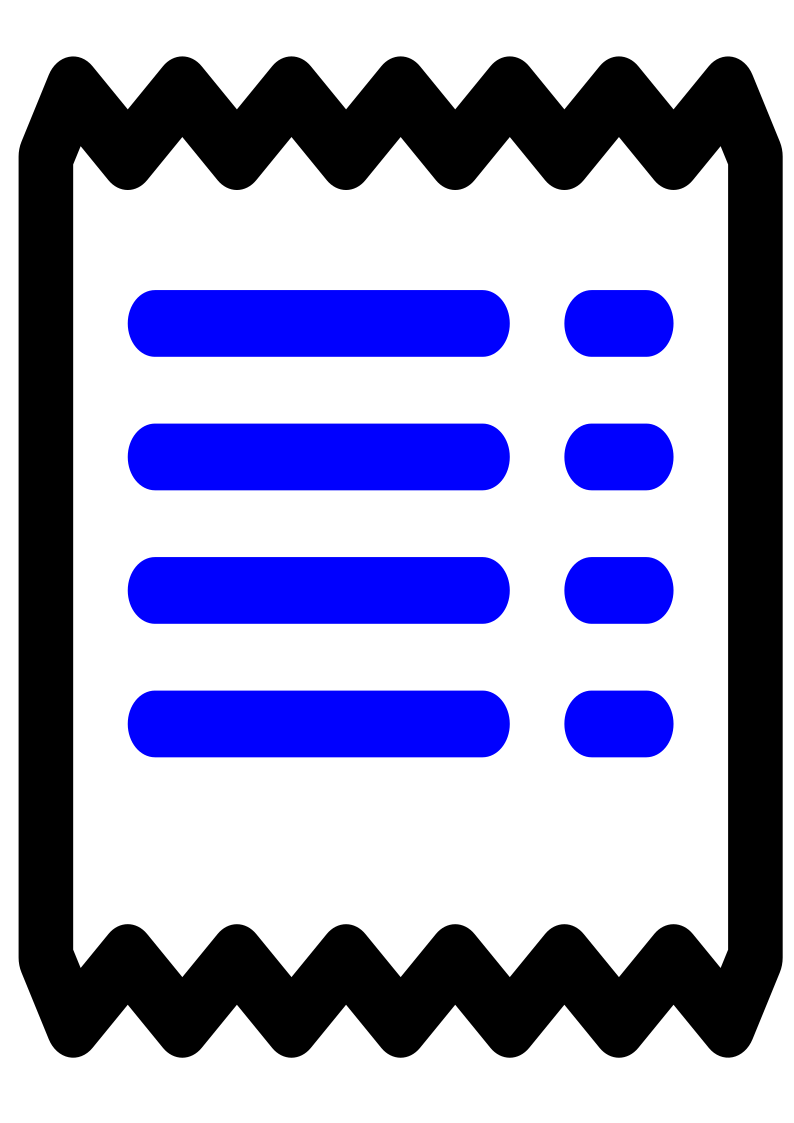
\includegraphics[width=0.9cm]{bilder/list_icon_2.png}\hspace{0.1cm}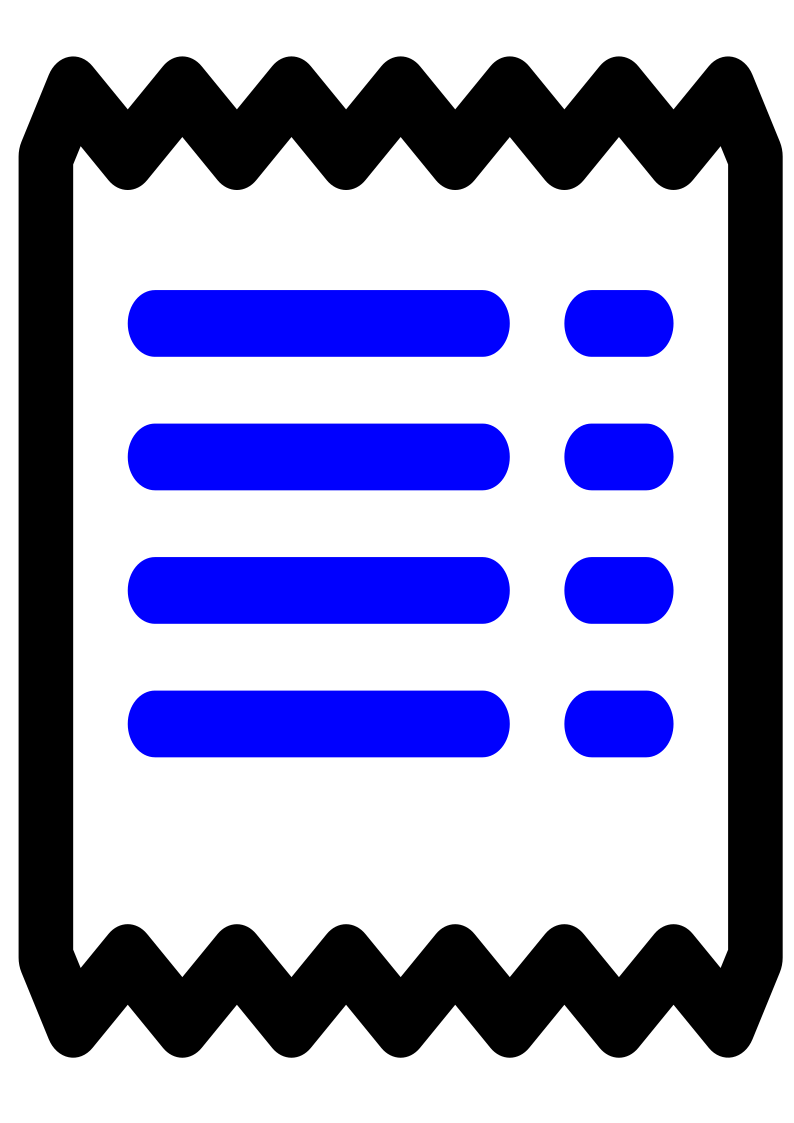
\includegraphics[width=0.9cm]{bilder/list_icon_2.png}\hspace{0.1cm}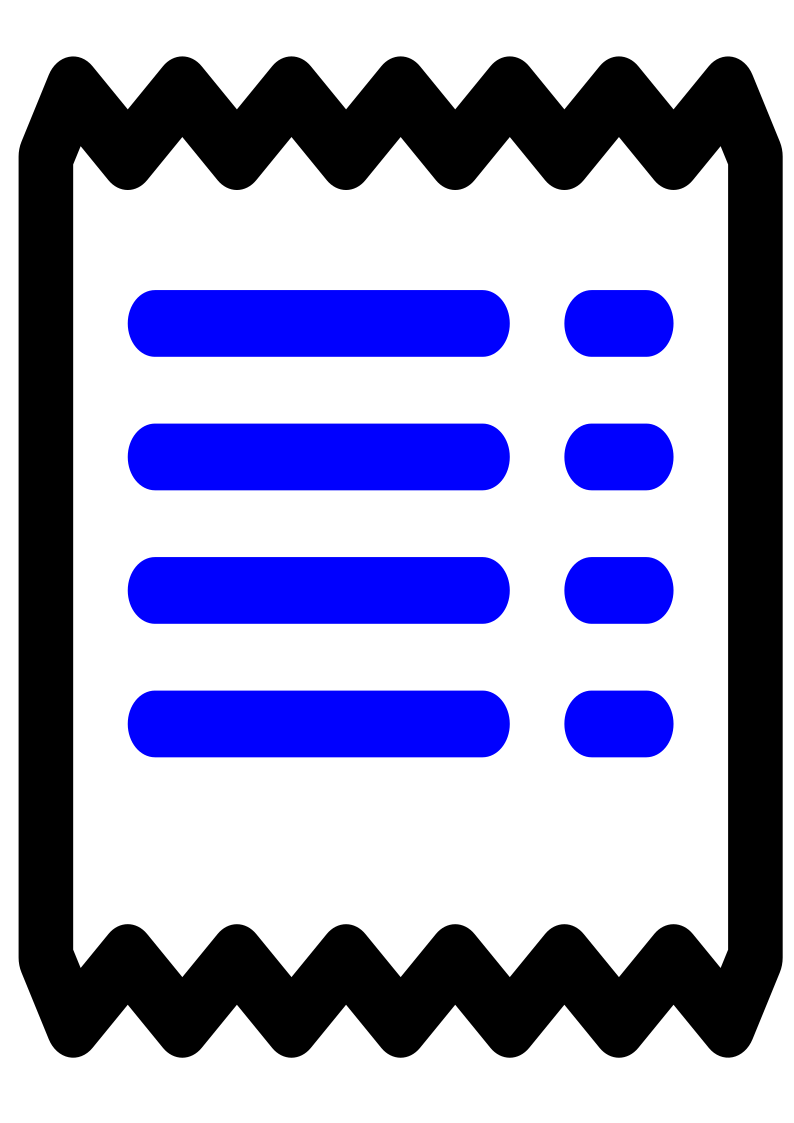
\includegraphics[width=0.9cm]{bilder/list_icon_2.png}};
		
		% Pfeile
		\path [line] (p15.south) -- node [above] {} (p16) ;     
		\path [line] (p16.south) -- node [above] {} (p17) ;
		\path [line] (p17.south) -- node [above] {} (p18) ;
		\path [line] (p18.south) -- node [above] {} (p19) ;		
		
		\path [dashedline] (p11.east) -- node [left] {} (p16.west);
		\path [dashedline] (p13.north) -- node [left] {} (p11.south); 
		
		\path (p11.north)+(0.0, 2.0) node (ur1)[ur] {\color{black}\lstinline|indicator_constrait()|};
		\path (p11.north)+(-0.0, 3.5) node (ur2)[ur] {\color{black}\lstinline|calc_loci_likelihoods()|};
		\path (p16.east)+(4.0, 0.0) node (ur3)[ur] {\color{black}\lstinline|get_heterozygosity()|};
		\path (ur3.north)+(0.0, 1.5) node (ur4)[ur] {\color{black}\lstinline|get_cigar_tuples()|};
		\path (p17.east)+(5.1, 0.0) node (ur5)[ur] {\color{black}\lstinline|get_allele_likelihood_alleles()|};
		
		\path [dashedline] (ur2.south) -- node [left] {} (ur1.north);
		\path [dashedline] (ur4.south) -- node [left] {} (ur3.north);
		
		% Pfeile%
		\draw [funtool] (p11.north) -- (ur1.south);		
		\draw [funtool] (p16.east) -- (ur3.west);	
		\draw [funtool] (p17.east) -- (ur5.west);
		
		\background{p2}{p16}{p4}{p18}{Loci Likelihood}
		\end{tikzpicture}
		\caption{Prozesse des Workflows - Likelihood der Loci-Zuordnung \cite{tikz_schema, bootstrap}}
		\label{fig:workflow_all}
	\end{center}
\end{figure}

In diesem Schritt sollen schließlich für die Allel-Fraction mit maximaler Likelihood (Kap. \ref{subsec:lh_allele}) die ermittelten Kandidatenloci (Kap. \ref{subsec:comb_loci}) unter Berücksichtigung der Heterozygotie analysiert werden und die wahrscheinlichste Kombination der Loci ermittelt werden.\\

Für jede Loci-Kombination aus \lstinline|get_candidate_loci()| wird aus der Funktion \linebreak \lstinline|calc_loci_likelihoods()| heraus zunächst geprüft, ob sich die Loci dieser Kombination der zuvor bestimmten Allelfraktion mit maximaler Likelihood zuordnen lassen. Dies geschieht mit Hilfe der Indikatorfunktion \hyperref[schritt14b]{\lstinline|indicator_constrait()|\phantomsection\label{schritt14btxt}} nach Formel \eqref{eqn:2-13}. Ist die Bedingung der Indikatorfunktion erfüllt, so wird die Likelihood der Loci-Kombination aus den Heterozygotiewahrscheinlichkeiten der darin enthaltenen Allele berechnet und zurückgegeben. Ist die Bedingung der Indikatorfunktion nicht erfüllt, so wird eine Likelihood von 0 zurückgegeben. Wie bereits besprochen, ist durch die Änderungen an der Implementierung von \lstinline|get_candidate_loci()| dieser Schritt nicht mehr notwendig und wurde nur belassen, um das dahinterstehende Modell strukturierter zeigen zu können.\\

Für die Likelihoodberechnung müssen nun einer Loci-Kombination zunächst die passenden Allelsequenzen zugeordnet werden. Die einzelnen Allele innerhalb einer Loci-Kombina-tion werden durch Integerwerte repräsentiert, die dem Index des dazugehörigen Kandidatenalleles entsprechen (siehe Kap. \ref{subsec:cand_allele}). Zu jeder Loci-Kombination wird also eine Liste $ S_{\,loc,\, alleles} $ generiert, welche die Kandidatenallelsequenzen der einzelnen Loci als Sublisten beinhaltet.\\

Die Berechnung der Likelihood ist im vorliegenden Modell zunächst nur für diploide Organismen möglich. Aanalog zur Likelihoodberechnung beim paarweisen Vergleich der Reads unter Berücksichtigung der Sequenzierfehlerwahrscheinlichkeit (Kap. \ref{subsec:edges}) erfolgt auch die Likelihoodberechnung für einer Loci-Kombination durch den paarweisen Vergleich der Allele im Sinne eines pair Hidden Markov Models $ pairHMM_{\eta}(a_{l_{j,1}}, a_{l_{j,2}}) $ (vgl. Kap. \ref{subsec:phmm_minimap}). Allerdings werden nun die Heterozygotiewahrscheinlichkeiten $\eta_{sub}$, $\eta_{ins}$ und $\eta_{del}$ der Grapheigenschaften zur Ermittlung der Likelihood nach Formel \eqref{eqn:2-12} genutzt.  \\

Hierzu werden zunächst in \hyperref[schritt16]{\lstinline|get_allele_likelihood_alleles()|\phantomsection\label{schritt16txt}} (Algorithmus \ref{alg:lh_loci}) auf jeweils einer der Listen $S_{\,loc,\, alleles}$ für jeden Locus $loc$ die darin enthaltenen Allelsequenzen $s_{a_{i}}, s_{a_{j}}$  der Allele ${a_{i}, a_{j}}$ paarweise mit einander kombiniert. Dies wird durch die Funktion \lstinline|combinations()| aus  \lstinline|itertools| realisiert, die Kombinationen ohne Wiederholung und ohne Beachtung der Reihenfolge erzeugt. Die paarweise Kombination der Allele ist allerdings nur für Daten diploider Organismen möglich, bei höherer Ploidie wird ein multiples Sequenzalignment benötigt (vgl. Kap \ref{sec:ausblick}). Für jedes Allelpaar werden dann die CIGAR-Tupel durch die Funktion \lstinline|get_cigar_tuples()| (Algorithmus \ref{alg:cig}) ermittelt und für die Likelihoodberechnung in \lstinline|get_heterozygosity()| verwendet (Algorithmus \ref{alg:lh_het}). Die Gesamtwahrscheinlichkeit errechnet sich aus dem Produkt der Likelihood aller Allelpaare nach \ref{eqn:2-14}. Analog zur Likelihoodberechnung der Allele (vgl. Algorithmus \ref{alg:r-a-lh}) werden auch die ermittelten Locilikelihoods für die verschiedenen Loci-Kombinationen mehrfach benötigt. Daher wird die Effizienz auch hier durch Integration eines Dictionary mit den bereits ermittelten Likelihoods deutlich erhöht. Die Einträge des Dictionary sollen dabei die Tupel aus den beiden Allelsequenzen als Keys und die bereits errechneten Likelihoods als Values verwenden. Für alle Allelsequenzpaare wird noch vor der Suche nach geeigneten CIGAR-Tupeln das Dictionary $ dict_{\,loc} $ auf bereits vorhandene Einträge überprüft.  Falls es einen Eintrag gibt, so wird auf eine erneute Likelihoodberechnung verzichtet und stattdessen der Wert des Dictionary verwendet. Falls kein Eintrag existiert, so wird im Anschluss an die Likelihoodberechnung ein entsprechender Eintrag dem Dictionary hinzugefügt.

\begin{algorithm}[H]
	\caption{Bestimmung der Likelihood der Allele innerhalb einer Loci-Kombination}  \label{alg:lh_loci}
	\begin{algorithmic}[1]	
		\Function{get\_allele\_likelihood\_alleles}{$ C_{k} $, $ S_{\,loc,\, alleles} $, $ dict_{\,loc} $}
		\State $ likelihood \gets 1.0 $
		\For{$ loc \in S_{\,loc,\, alleles} $}
		    \State $ pairs \gets combinations(loc) $
		    \algorithmiccomment{\href{https://docs.python.org/3/library/itertools.html\#itertools.combinations}{itertools.combinations()}}
		    \For{$ (s_{a_{i}}, s_{a_{j}}) \in pairs $}
		    \If{$\exists (s_{a_{i}}, s_{a_{j}}): ((s_{a_{i}}, s_{a_{j}}), L_{a_{i}, a_{j}}) \in dict_{\,loc}$}
		    \State $likelihood \gets likelihood + L_{a_{i}, a_{j}} $

		    \Else
		    
		    
		    
		    \State $cigar \gets get\_cigar\_tuples(C_{k}, s_{a_{i}}, s_{a_{j}})$  \algorithmiccomment{Alg. \ref{alg:cig}}
			    \If{$cigar$ exists}
			        \State $cig \gets cigar\,[\,0\,]$
			        \State $rev \gets cigar\,[\,1\,]$
			        \State $ \eta_{rates} \gets C_{k}[\eta_{sub}] \cup C_{k}[\eta_{ins}] \cup C_{k}[\eta_{del}]$
			        \State $L_{a_{i}, a_{j}} \gets log(get\_heterozygosity(\eta_{rates}, cig, rev))$  \algorithmiccomment{Alg. \ref{alg:lh_het}}
			        \State $ dict_{\,loc} \gets dict_{\,loc} \, \cup ((s_{a_{i}}, s_{a_{j}}),  L_{a_{i}, a_{j}})  $
			    	\State $ likelihood \gets likelihood + L_{a_{i}, a_{j}}$    
			        \EndIf
			\EndIf
			\EndFor
		\EndFor
		\State \Return $ e^{\;likelihood} $
		\EndFunction
	\end{algorithmic}
\end{algorithm}

In \hyperref[schritt15]{\lstinline|get_heterozygosity()|\phantomsection\label{schritt15txt}} erfolgt die Likelihoodberechnung der paarweisen Kombinationen der Allelsequenzen eines Locus aus den CIGAR-Tupeln und den Heterozygotiewahrscheinlichkeiten. Dies beschränkt den Prototypen derzeit auf diploide Organismen (siehe auch Kap. \ref{sec:ausblick}). Wie in Algorithmus \ref{alg:lh_read} wird auch hier die Likelihood über aller Matches und Mismatches aus den Informationen der CIGAR-Tupel bestimmt. Die Likelihoodberechnung der Matches erfolgt dabei nach Formel \ref{eqn:2-5}, die der Mismatches nach Formel \ref{eqn:2-6}. Das Argument \lstinline|reverse| markiert zudem die Richtung der Kante, von der die CIGAR-Tupel stammen. Für  Kanten in Rückrichtung, die von der Referen- zur Query-Sequenz verlaufen gilt \lstinline|reverse=True|. In diesem Fall werden Deletionen als Insertionen behandelt und umgekehrt. \\

\begin{algorithm}[H]
	\caption{Bestimmung der Likelihood zwischen zwei Kandidatenallelen hinsichtlich der Heterozygotiewahrscheinlichkeiten}  \label{alg:lh_het}
	\begin{algorithmic}[1]	
		\Function{get\_heterozygosity}{$\eta_{sub}$, $\eta_{ins}$, $\eta_{del}$, $ cigar\_tuples $, $ reverse $}
		\State $likelihood \gets 1.0$
		\If{reverse}
		\State swap values of $\eta_{ins}$ and $\eta_{del}$
		\EndIf
		\ForAll{$(operation, length) \in cigar\_tuples$}
		\If{$operation \in match$}
		\State $ likelihood \gets likelihood \, \cdotp (1 - (\eta_{sub}+\eta_{ins}+\eta_{del}))^{\;length} $
		\EndIf		    		    	
		\If{$operation \in substitution$}
		\State $likelihood \gets likelihood \, \cdotp (\eta_{sub})^{length}$
		\EndIf	
		\If{$operation \in insertion$}
		\State $likelihood \gets likelihood \, \cdotp (\eta_{ins})^{length}$
		\EndIf
		\If{$operation \in deletion$}
		\State $likelihood \gets likelihood \, \cdotp (\eta_{del})^{length}$
		\EndIf
		\EndFor
		\State \Return $ likelihood $
		\EndFunction
	\end{algorithmic}
\end{algorithm}

Wie bereits erwähnt, werden für den paarweisen Vergleich zweier Kandidatenallele im Rahmen der Likelihoodberechnung die dazugehörigen CIGAR-Tupel benötigt. Diese werden durch die Funktion \lstinline|get_cigar_tuples()| ermittelt. Als Eingabeparameter erhält die Funktion den Subgraphen der Zusammenhangskomponente sowie die beiden Kandidatenallelsequenzen: die Query-Sequenz $ s_{source} $ und die Referenz-Sequenz $ s_{target} $. Der Subgraph wird nach einer Kante durchsucht, die Knoten miteinander verbindet, welche die beiden gegebenen Sequenzen besitzen. Dabei werden nicht nur Kanten berücksichtigt, die von der Query- zur Referenzsequenz verlaufen, sondern auch Kanten in Gegenrichtung. Zur Markierung der Kantenrichtung gibt die Funktion neben den CIGAR-Tupeln auch einen booleschen Wert zurück. Dieser wird in der Funktion \lstinline|get_heterozygosity()| (Kap. \ref{subsec:lh_loci}) für das Argument \lstinline|reverse| verwendet. \\

Um eine passende Kante im Subgraphen zu finden, erstellt \lstinline|get_cigar_tuples()| zunächst eine Liste aller Knoten $ R_{source} = (v_{1}, \dots, v_{i})$, welche die Query-Sequenz $ s_{query} $ besitzen sowie eine Liste aller Knoten $ R_{target} = (w_{1}, \dots, w_{j}) $, die die Referenz-Sequenz $ s_{ref} $ tragen. Hierfür werden für beide Sequenzen die Knoten des Subgraphen mit \lstinline|find_vertex()| aus graph-tool durchsucht. Anschließend wird nach einer Kante gesucht, die einen der Knoten aus $ R_{source} $ mit einem der Knoten aus $ R_{target} $ verbindet. Es erfolgt also ein Kantenaufruf für jeden Knoten aus $ R_{source} $ in Kombination mit jedem  Knoten aus $ R_{target} $. Der Kantenaufruf wird sowohl für die angegebene Kantenrichtung und falls erfolglos auch für die entgegengesetzte Richtung durchgeführt. Existiert eine solche Kante, dann werden die CIGAR-Tupel sowie der boolsche Wert entsprechend der Kantenrichtung zurückgegeben, andernfalls wird $ None $ zurückgegeben. \\

Zur Veranschaulichung ist der Algorithmus in \ref{alg:cig} zudem als Pseudocode dargestellt. Dabei sei $ C_{k} \in \{C_{1}, \dots ,C_{p}\} $ der Subgraph einer Zusammenhangskomponente mit seiner Kantenmenge $ E_{k} $ und $ s_{query} $ bzw. $ s_{ref} $ seien die Query- bzw. die Referenz-Sequenz. Die Verwendung fester Knoten- oder Kanteneigenschaften ist durch eckige Klammern gekennzeichnet, so ruft beispielsweise $v_{i}[sequence]$ die Sequenz des Knotens $v_{i}$ aus den Knoteneigenschaften ab. \\

\begin{algorithm}[H]
	\caption{CIGAR-Tupel bestimmen}  \label{alg:cig}
	\begin{algorithmic}[1]	
		\Function{get\_cigar\_tuples}{$ C_{k} $, $ s_{query} $, $ s_{ref} $}
		\State $ R_{source} \gets \{v_{i} \in C_{k} \wedge i,k \in \mathds{N} \; |\; v_{i}[sequence]= s_{query} \}$
		\State $ R_{target} \gets \{w_{j} \in C_{k} \wedge j,k \in \mathds{N} \; |\; w_{j}[sequence]= s_{ref} \}$
		\For{$ v_{i} \in R_{source} $}
		\For{$ w_{j} \in R_{target} $}
		\If{$ (v_{i}, w_{j}) \in E_{k}$}
		\State \Return $ (\;E_{k}[(v_{i}, w_{j})][cigar\_tuples],\, False\;) $		    
		\EndIf
		\If{$ (w_{j}, v_{i}) \in E_{k}$}
		\State \Return $ (\;E_{k}[(w_{j}, v_{i})][cigar\_tuples],\, True\;) $		
		\EndIf
		\EndFor
		\EndFor
		\State \Return $ None $
		\EndFunction
	\end{algorithmic}
\end{algorithm}

In \lstinline|noderad_main.py| werden die beschriebenen Schritte zur Likelihoodberechnung für alle Permutationen ausgeführt und anschließend die Loci-Kombination mit \hyperref[schritt17]{maximaler Likelihood\phantomsection\label{schritt17txt}} als wahrscheinlichste Loci-Verteilung ausgewählt.\\

In den Log-Dateien werden zusätzlich einige Statistiken zur Berechnung der wahrscheinlichsten Loci-Verteilung eingetragen. Dazu gehören die ermittelten Likelihoods der Loci-Kombination sowie die Loci mit maximaler Likelihood. \\

\section{Ausgabe der wahrscheinlichsten Loci als VCF-Datei} \label{sec:vcf}

\begin{figure}[h]
	\begin{center}
		\begin{tikzpicture}[scale=0.64,transform shape]
		\path (p17.south)+(0.0,-1.3) \ioitem{18}{17. Maximum likelihood loci};
		\path (p18.south)+(0.0,-1.7) \blockitem{19}{\hyperref[schritt18txt]{\color{white}..}18.\phantomsection\label{schritt18} VCF \\ 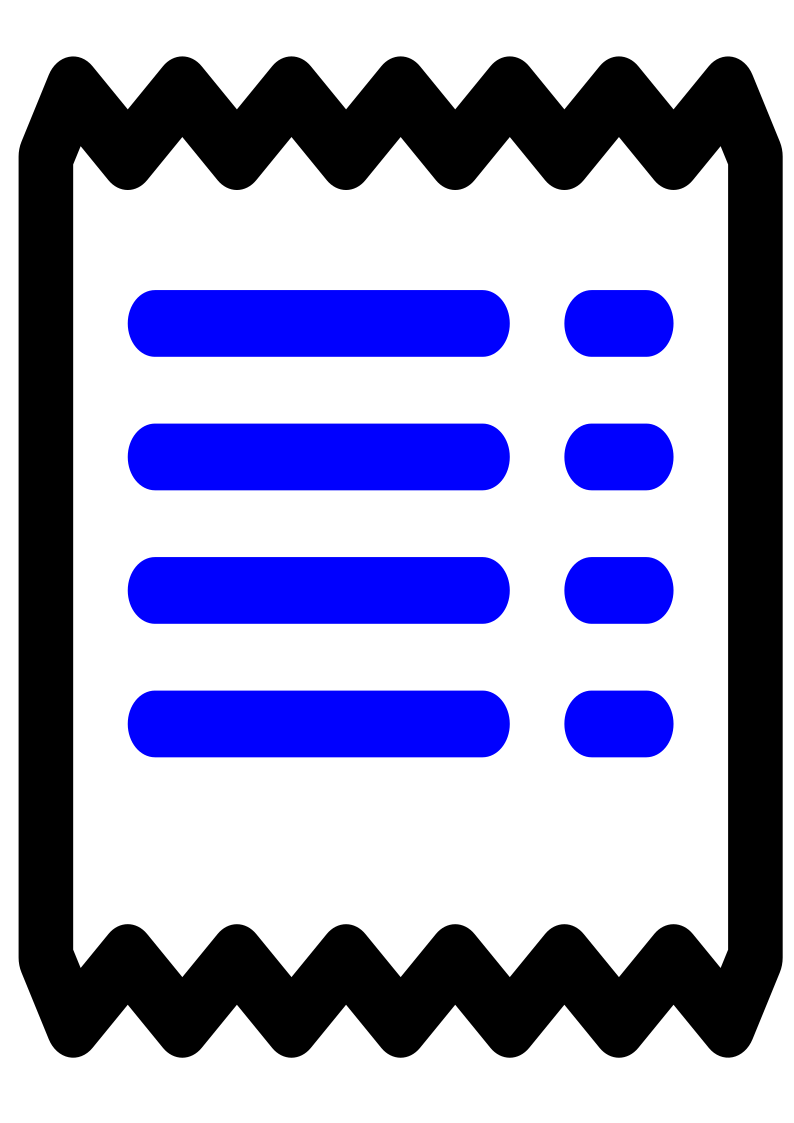
\includegraphics[width=0.9cm]{bilder/list_icon_2.png}\hspace{0.1cm}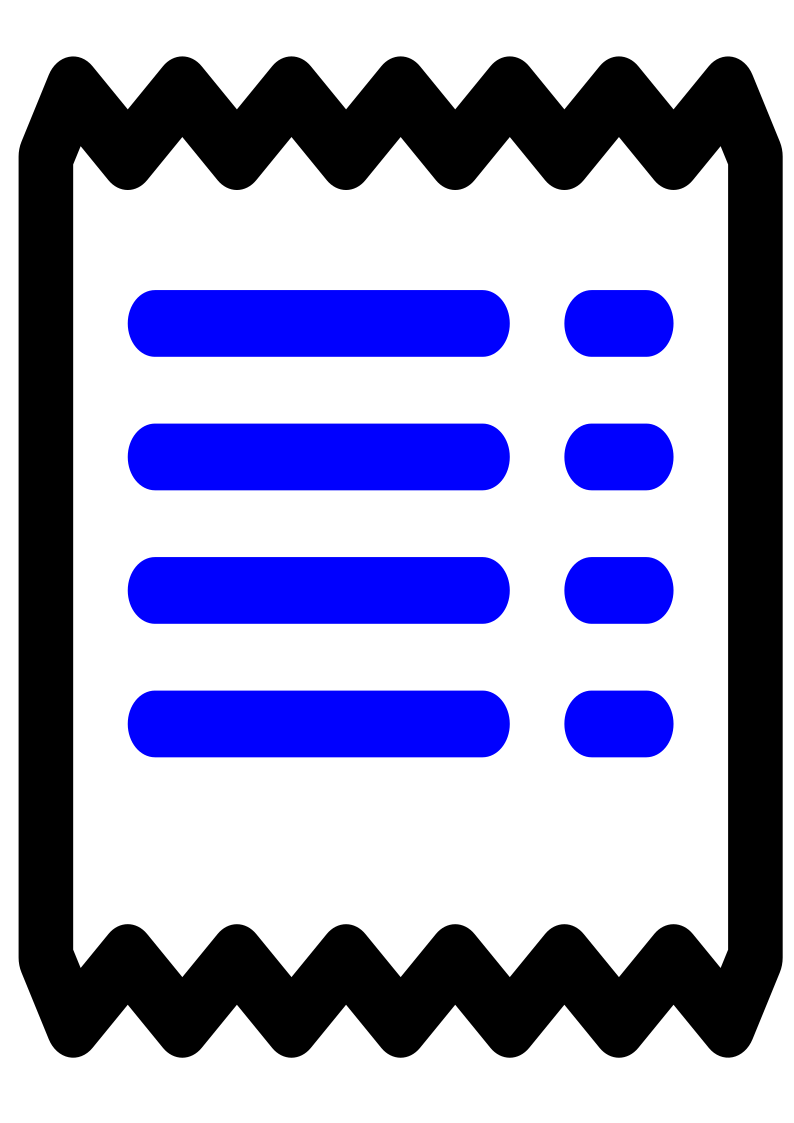
\includegraphics[width=0.9cm]{bilder/list_icon_2.png}\hspace{0.1cm}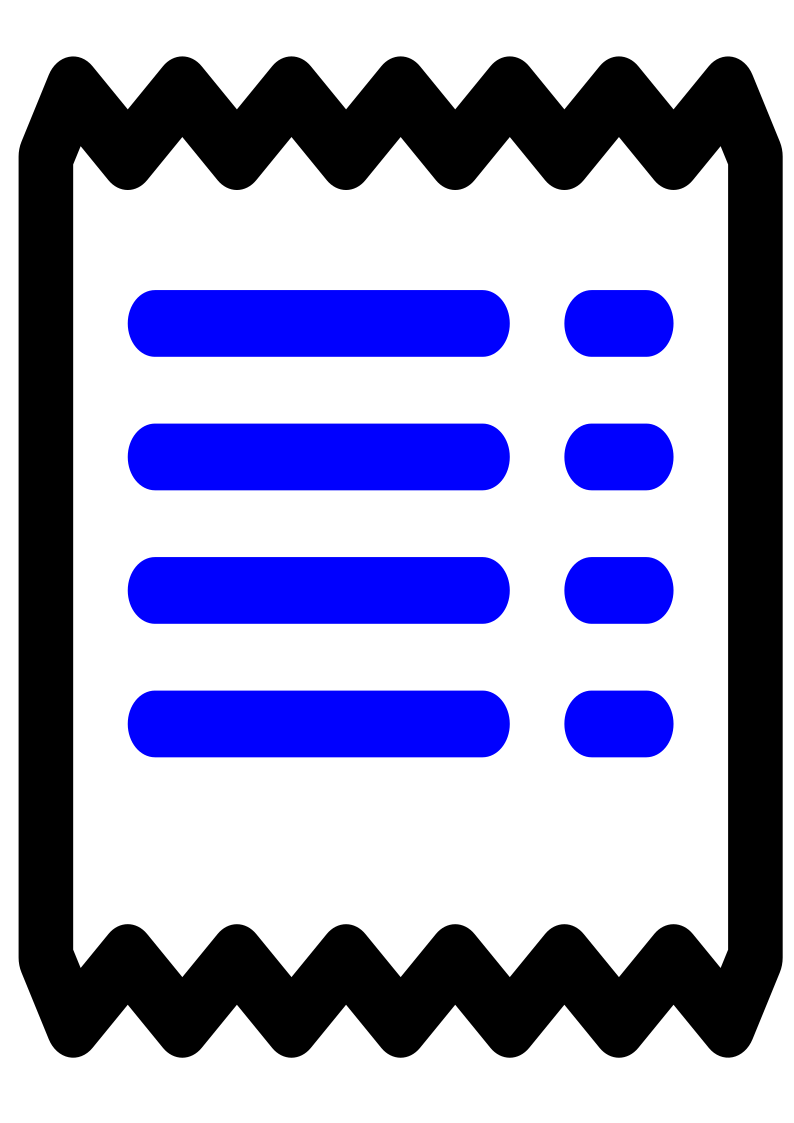
\includegraphics[width=0.9cm]{bilder/list_icon_2.png}};
		\path (p19.west)+(-4.1, 1.0) node (ur1)[ur] {\color{black}\lstinline|get_sorted_loci_alleles()|};
		\path (p19.west)+(-4.5, 0.0) node (ur2)[ur] {\color{black}\lstinline|get_alleles_matched_to_loci()|};
		\path (p19.west)+(-3.21, -1.0) node (ur3)[ur] {\color{black}\lstinline|get_gt_indices()|};
		\path (p19.west)+(-3.03, -2.0) node (ur4)[ur] {\color{black}\lstinline|get_genotype()|};
		
		% Pfeile
		\path [line] (p18.south) -- node [above] {} (p19) ;		
		
		\draw [funtool] (p19.west) -- (ur1.east);
		\draw [funtool] (p19.west) -- (ur2.east);
		\draw [funtool] (p19.west) -- (ur3.east);
		\draw [funtool] (p19.west) -- (ur4.east);
		
		\background{p18}{p18}{p18}{p18}{Loci Likelihood}
		\end{tikzpicture}
		\caption{Prozesse des Workflows - Ausgabe als VCF-File \cite{tikz_schema, bootstrap}}
		\label{fig:workflow_all}
	\end{center}
\end{figure}

Die Loci-Kombinationen mit maximaler Likelihood $Loc_{max}$ aller Zusammenhangskomponenten werden für jedes Individuum jeweils in eine Datei im \hyperref[schritt18]{Variant Call Format\phantomsection\label{schritt18txt}} (siehe Kap. \ref{subsec:vcformat}) geschrieben. Dabei werden zusätzlich die optionalen FORMAT- und Proben-Spalten zur Kennzeichnung des Genotyps verwendet. \\

In die Spalten REF und ALT werden die Sequenzen der Allele aus $Loc_{max}$ lexikographisch sortiert eingetragen. Hierfür wird in der Funktion \lstinline|get_sorted_loci_alleles()| eine sortiere Liste der Allelsequenzen aus $Loc_{max}$ gebildet. Durch die Pythonfunktion \lstinline|set()| wird über dieser Liste die Menge der Allele extrahiert, so dass Duplikate herausgefiltert werden. Aus der so entstandenen Liste der Allelsequenzen $A_{res}$ wird der erste Eintrag in die Spalte REF eingetragen, die übrigen Einträge werden in die Spalte ALT geschrieben.\\

Da jeweils die vollständige Sequenz der Allele für den Eintag in die VCF-Datei verwendet wird, wird für jeden Locus in der Spalte POS der Wert $1$ eingetragen. \\

In der FORMAT-Spalte wird durch den Eintrag ``GT'' festgelegt, dass in der Probenspalte der Genotyp spezifiziert wird. Da die Indizes der Loci der Liste der Kandidatenallele zugeordnet sind, aber nicht alle Allele dieser Liste auch in $Loc_{max}$ vorkommen, muss ihre Indizierung nun auf die bereits erstellte Liste mit den zu $Loc_{max}$ gehörigen Allelsequenzen $A_{res}$ angepasst werden. \\

Hierfür werden in der Funktion \lstinline|get_alleles_matched_to_loci()| zunächst jedem Locus aus $Loc_{max}$ die entsprechenden Sequenzen aus der Liste der Kandidatenallele zugeordnet. Anschließend werden diese Sequenzen in \lstinline|get_gt_indices()| den Indizes der passenden Sequenz aus $A_{res}$ zugeordnet. Dadurch wird das lexikographisch erste Allel, also REF mit 0 im Genotyp indiziert, die Allele aus ALT erhalten höhere Indizes entsprechend ihrer Sortierung in $A_{res}$. Nun lässt sich der Genotyp im Bezug auf die Sequenzen in REF und ALT aus diesen Indizes und getrennt durch Slashes direkt angeben. Dies geschieht in der Funktion \lstinline|get_genotype()|, deren Ergebnis dann in die Probenspalte eingetragen wird.\\
\let\cleardoublepage\clearpage

